\chapter{Resultados e Validação} \label{ch:results}

Com o simulador finalizado, é necessária a avaliação de seus resultados para que a implementação seja validada. A apresentação e a análise de simulações são feitas neste capítulo. Com o fim de se fazer a validação numérica, os resultados são comparados com soluções analíticas ou qualitativamente avaliados.

O procedimento adotado para validação numérica da implementação considera:
\begin{alineas}
	\item a análise qualitativa da solução numérica. Por exemplo, em simulações sem forças externas, as quantidades de movimento linear e angular devem se manter constantes no sistema, e a verificação desse fato no resultado da simulação indica, nesse sentido, uma representatividade correta do fenômeno físico estudado;
	\item a comparação qualitativa com a solução analítica, se esta estiver disponível. Este item é semelhante ao anterior, mas considera ainda a solução analítica para o estudo do comportamento dos resultados numéricos; 
	\item o estudo do erro da solução numérica com relação à analítica, se esta for conhecida. O erro representa o grau de discordância entre as soluções, e valores baixos indicam a corretude do algoritmo.
\end{alineas}


O \textit{erro} de um resultado é uma medida fundamental para atestar-se a validade do método. Quanto maior o erro, menos representativa se torna a simulação. Sendo \(y\) uma solução obtida numericamente e \(\analytical{y}\) a solução exata do problema, define-se o erro de \(y\) como
\begin{equation*}
	\errorOf{y} = \abs{y - \analytical{y}}.
\end{equation*}

O erro máximo, por sua vez, é o maior erro pontual entre \(y\) e \(\analytical{y}\), isto é, é o maior elemento do conjunto imagem da função erro:
\begin{equation*}
	\maximumErrorOf{y} = \max\pqty{\Im\pqty{\errorOf{y}}}.
\end{equation*}

Para funções vetoriais \(\vec{y}\), o erro e o erro máximo são definidos equivalentemente como
\begin{gather}
	\errorOf{\vec{y}} = \norm{\vec{y} - \analytical{\vec{y}}}, \label{eq:vector_error} \\
	\maximumErrorOf{\vec{y}} = \max\pqty{\Im\pqty{\errorOf{\vec y}}}. \label{eq:maximum_vector_error}
\end{gather}

Todas as simulações foram executadas em um computador com épsilon de máquina aproximadamente igual a \(2\cdot10^{-16}\), memória \RAM{} de 16\GiB{} e processador Intel Core i7-4770 \SI{3.40}{\giga\hertz}.

Foram escolhidos quatro problemas a serem apresentados e estudados: o problema do lançamento oblíquo, em que uma partícula é lançada no espaço sujeita unicamente à ação da gravidade; o problema da esfera quicando, em que uma partícula liberada no espaço em repouso é atraída, pela gravidade, em direção ao chão, colidindo com ele; a colisão com rotação, em que duas esferas se chocam, sendo que uma delas possui velocidade angular não nula; e o problema da queda com arrasto, em que uma partícula é solta no espaço e cai em decorrência da ação da gravidade, sofrendo, ao longo de sua trajetória, a resistência do ar.

\section{Lançamento Oblíquo} \label{sec:free_fall}

O lançamento oblíquo é um dos problemas clássicos de física básica. Considera-se uma partícula de massa \(\mass\) sujeita unicamente à ação de um campo gravitacional constante cuja aceleração da gravidade é \(\gravity\). Nessas condições, as equações de movimento para a partícula se tornam, simplesmente,
\begin{gather}
	\acceleration = \gravity, \label{eq:free_fall_translation}\\
	\angularAcceleration = \nullVector \label{eq:free_fall_rotation}.
\end{gather}

\alert{Dizer que a solução é trivial e tirar essa dedução}

O instante inicial da simulação é definido como \(\initialInstant=0\), e o instante final é um valor arbitrário \(\finalInstant\). A posição, a velocidade e a velocidade angular da partícula no instante inicial assumem, respectivamente, os valores \(\initial{\position}\), \(\initial{\velocity}\) e \(\initial{\angularVelocity}\). Com isso, as equações \eqref{eq:free_fall_translation} e \eqref{eq:free_fall_rotation} podem ser resolvidas por integração simples:
\begin{gather*}
	\acceleration\pqty{t} = \gravity, \\
	\velocity\pqty{t} = \initial{\velocity} + \int_{\initialInstant}^{t} \acceleration\pqty{\tau} \dd{\tau} = \initial{\velocity} + \gravity\cdot t, \\
	\position\pqty{t} = \initial{\position} + \int_{\initialInstant}^{t} \velocity\pqty{\tau} \dd{\tau} = \initial{\position} + \initial{\velocity}\cdot t + \gravity\cdot \dfrac{t^2}{2}, \\
	\angularVelocity\pqty{t} = \initial{\angularVelocity} + \int_{\initialInstant}^{t} \nullVector \dd{\tau} = \initial{\angularVelocity}.
\end{gather*}

Por simplicidade, considera-se que o movimento ocorra apenas no plano \(\xAxis\yAxis\), que a gravidade atue no sentido negativo do eixo \(\yAxis\), isto é, \(\gravity = -\gravityScalar\cdot\yUnit\) com \(\gravityScalar>0\), e que a partícula não possua rotação, como representado na figura \ref{fig:free_fall}. Nessa situação, a posição em \(\yAxis\) da partícula é chamada de altura.

\begin{figure}[h]
	\caption{O problema do lançamento oblíquo}
	% \vspace{-0.5cm}
	\centering
		\alert{Colocar imagem representando o problema do lançamento oblíquo}
		% 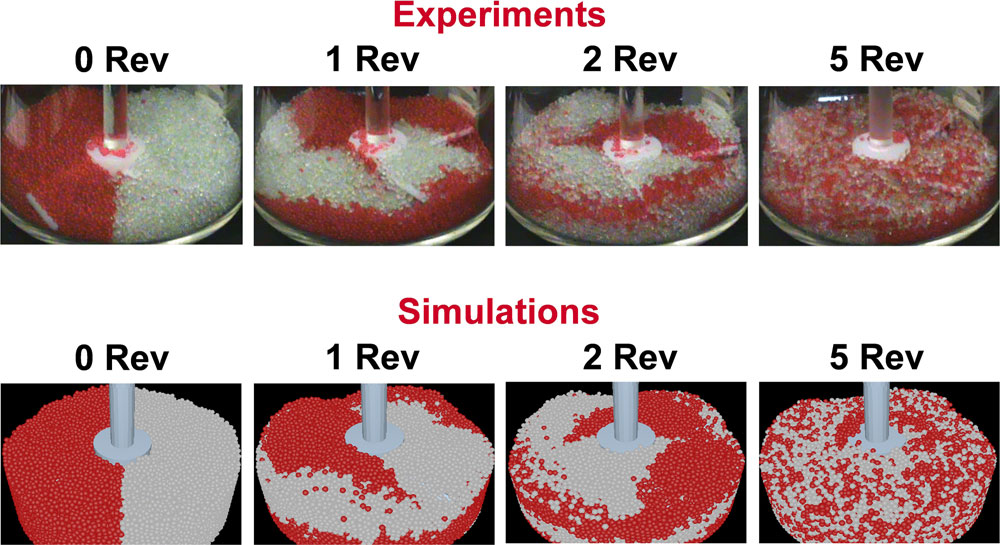
\includegraphics[width=0.65\textwidth]{images/drug_production.png}
	% {\centerline{\includegraphics[scale=#2]{#1}}}
	% \vspace{-0.2cm}
	\label{fig:free_fall}
	\source{\alert{Citar fonte}}
	% \vspace{-1cm}
\end{figure}

Com isso, escrevendo \(\position = \explicitVectorCoordinates{\positionScalar}\), \(\velocity = \explicitVectorCoordinates{\velocityScalar}\) e \(\acceleration = \explicitVectorCoordinates{\accelerationScalar}\), é obtida a solução como apresentada na tabela \ref{table:free_fall_solution}.

\begin{table}[h]
	\caption{Solução do problema do lançamento oblíquo}
	\label{table:free_fall_solution}

	\begin{equation*}
		\arraycolsep=1.5\arraycolsep
		\def\arraystretch{1.5}
		\begin{array}{lcc}
	\hline
		& \text{Direção } \xAxis 
		& \text{Direção } \yAxis \\
	\text{Posição} 
		& \positionx = \initial{\positionx} + \initial{\velocityx}\cdot \Dt
		& \positiony = \initial{\positiony} + \initial{\velocityy}\cdot \Dt - \dfrac{\gravityScalar\Dt^2}{2} \\
	\text{Velocidade} 
		& \velocityx = \initial{\velocityx}
		& \velocityy = \initial{\velocityy} - \gravityScalar\cdot \Dt \\
	\text{Aceleração} 
		& \accelerationx = 0
		& \accelerationy = - \gravityScalar \\
	\hline	
		\end{array}
	\end{equation*}
	\sourceMe
\end{table}

Embora seja conceitualmente simples e de fácil resolução, o problema do lançamento oblíquo permite:
\begin{itemize}
\item A validação numérica da implementação do algoritmo de Gear em simulações sem colisões, mas com a atuação de forças de campo. Em cada instante, as coordenadas da partícula são previstas e, em seguida, corrigidas a partir do valor da força da gravidade. A proximidade da resposta numericamente calculada com a solução analítica evidencia o bom funcionamento do algoritmo.
\item A obtenção da evolução do erro com o tempo de simulação. Não só existe um erro associado ao método como esse erro se acumula com o tempo.
\end{itemize}

A fim de se compararem os resultados numéricos com a solução analítica, foram arbitrados aos parâmetros do problema os valores dispostos na tabela \ref{tab:free_fall_case_parameters}.

\begin{table}[h]
\centering
\caption{Parâmetros para o problema de lançamento oblíquo.}
\label{tab:free_fall_case_parameters}
\begin{parametersdesc}
	\item{Gravidade}{\gravityScalar = 9,81}{\si[per-mode=symbol]{\metre\per\square\second}}
	\arrayrulecolor[gray]{0.8}\hline
	\item{Massa da partícula}{\mass = 1}{\si\kilogram}
	\item{Raio da partícula}{\radius = 3}{\si\centi\metre}
	\item{Posição inicial}{\explicitVector{\initial{\positionx}}{\initial{\positiony}}{\initial{\positionz}} = \explicitNumericVector{0}{0}{0}}{\si{\metre}}
	\item{Velocidade inicial}{\explicitVector{\initial{\velocityx}}{\initial{\velocityy}}{\initial{\velocityz}} = \explicitNumericVector{20}{10}{0}}{\si[per-mode=symbol]{\metre\per\second}}
	\item{Aceleração inicial}{\explicitVector{\initial{\accelerationx}}{\initial{\accelerationy}}{\initial{\accelerationz}} = \explicitNumericVector{0}{-9,81}{0}}{\si[per-mode=symbol]{\metre\per\square\second}}
	\arrayrulecolor[gray]{0.8}\hline
	\item{Instante final}{\finalInstant = 3}{\si\second} 
	\item{Passo de tempo}{\Dt = 10^{-3}}{\si\second}
	\item{Ordem de extrapolação}{\taylorOrder = 7}{\emptyUnit}
	\arrayrulecolor{black}
\end{parametersdesc}
\sourceMe 
\end{table}

Muito embora se trate de um problema bidimensional sem rotação, o simulador utiliza a formulação tridimensional e considera a evolução da velocidade angular da partícula.

\begin{figure}[htb!]
	\caption{Solução para a altura da partícula no problema de lançamento oblíquo\protect\footnotemark.}
	% \vspace{-0.5cm}
	\centering
		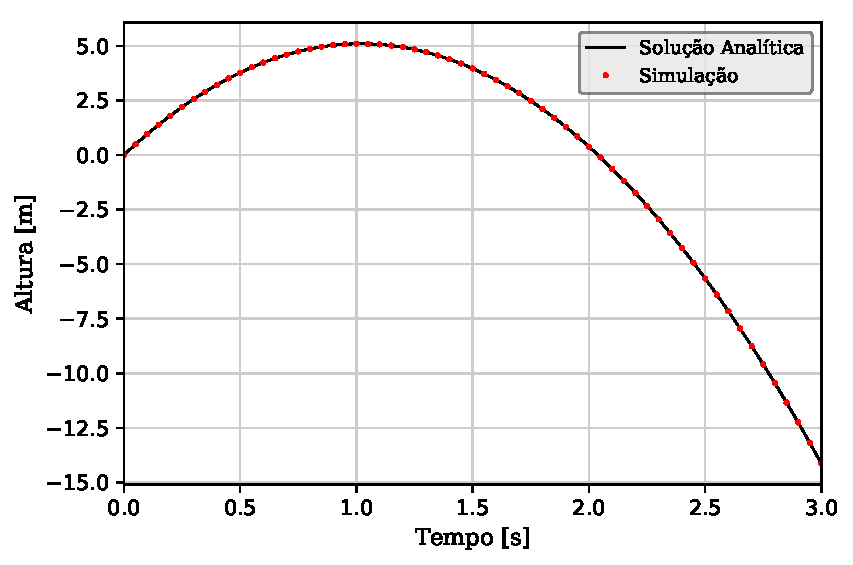
\includegraphics[scale=1]{images/falling_sphere/correct_initial_acceleration/y_position.pdf}
		% 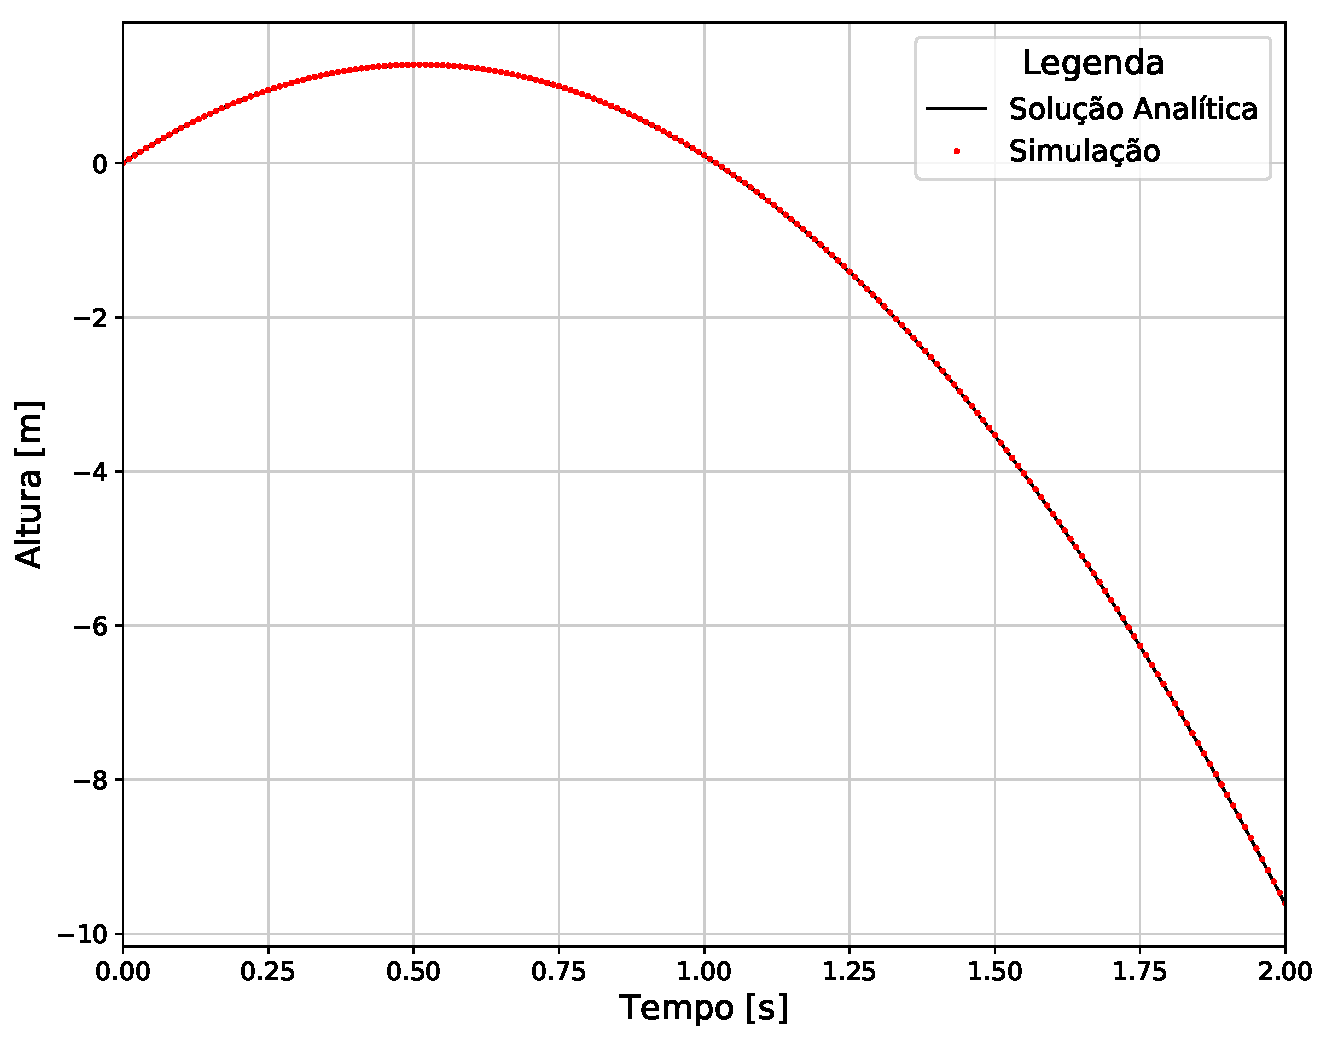
\includegraphics[width=\normalresultsfigwidth]{images/falling_sphere/y_position.pdf}
	% {\centerline{\includegraphics[scale=#2]{#1}}}
	% \vspace{-0.2cm}
	\label{fig:falling_sphere_y_position}
	\sourceMe
	% \vspace{-1cm}
\end{figure}

\footnotetext{Para melhor visualização dos resultados, é apresentado apenas um ponto a cada dez passos de tempo.}

\begin{figure}[htb!]
	\caption[Solução do problema de lançamento oblíquo para a posição horizontal, a velocidade horizontal, a velocidade vertical e a aceleração vertical da partícula]{Solução do problema de lançamento oblíquo para (\subref{subfig:x_position}) a posição horizontal, (\subref{subfig:x_velocity}) a velocidade horizontal, (\subref{subfig:y_velocity}) a velocidade vertical e (\subref{subfig:y_acceleration}) a aceleração vertical da partícula}
	% \vspace{-0.5cm}
	\centering
	\captionsetup[subfloat]{labelfont=bf}
	\subfloat{
		\centering
		\begin{subfigure}[t]{\smallresultsfigwidth}
			\centering
			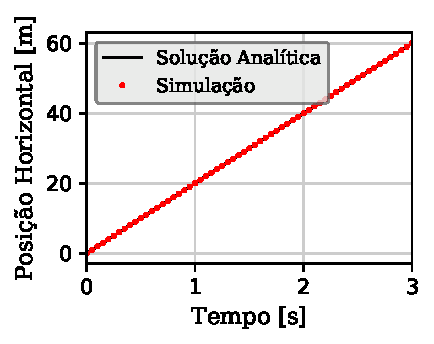
\includegraphics[scale=1]{images/falling_sphere/correct_initial_acceleration/x_position.pdf}
			\caption{}
			\label{subfig:x_position}
		\end{subfigure}
		\begin{subfigure}[t]{\smallresultsfigwidth}
			\centering
			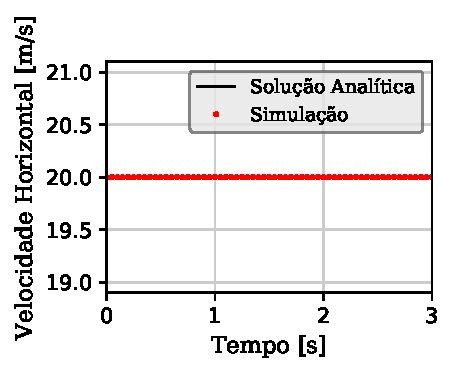
\includegraphics[scale=1]{images/falling_sphere/correct_initial_acceleration/x_velocity.pdf}
			\caption{}
			\label{subfig:x_velocity}
		\end{subfigure}
		\begin{subfigure}[t]{\smallresultsfigwidth}
			\centering
			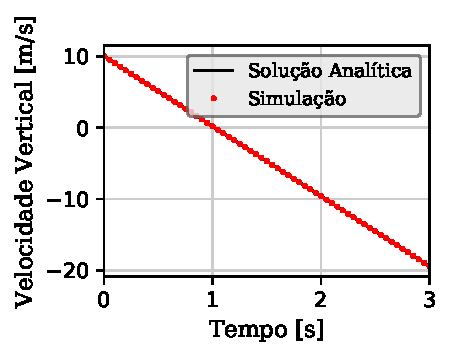
\includegraphics[scale=1]{images/falling_sphere/correct_initial_acceleration/y_velocity.pdf}
			\caption{}
			\label{subfig:y_velocity}
		\end{subfigure}
		\begin{subfigure}[t]{\smallresultsfigwidth}
			\centering
			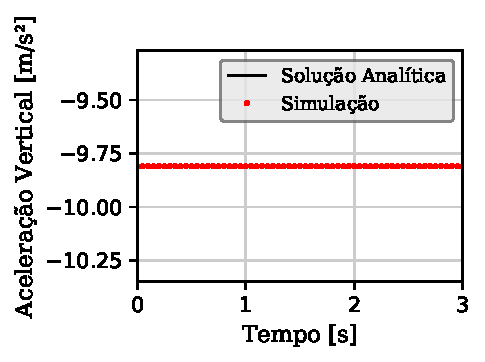
\includegraphics[scale=1]{images/falling_sphere/correct_initial_acceleration/y_acceleration.pdf}
			\caption{}
			\label{subfig:y_acceleration}
		\end{subfigure}
	}
	% \vspace{-0.2cm}
	\label{fig:falling_sphere_other}
	\sourceMe
	% \vspace{-1cm}
\end{figure}

Com esses parâmetros, foi calculada a trajetória da partícula através do simulador e da solução analítica. Na \cref{fig:falling_sphere_y_position} estão expostas as soluções para a altura da partícula. Observa-se nessa figura que os resultados obtidos pelo simulador se aproximam bastante da solução analítica das equações.

Outras variáveis, como a posição horizontal, as velocidades horizontal e vertical e a aceleração vertical estão apresentadas na \cref{fig:falling_sphere_other}.

\begin{figure}[htb!]
	\caption[Erro da simulação com relação à solução numérica para a posição e da partícula do problema do lançamento oblíquo]{Erro da simulação com relação à solução numérica para (\subref{subfig:position_error}) a posição e (\subref{subfig:velocity_error}) da partícula do problema do lançamento oblíquo}
	% \vspace{-0.5cm}
	\centering
	\captionsetup[subfloat]{labelfont=bf}
	\subfloat{
		\centering
		\begin{subfigure}[t]{\smallresultsfigwidth}
			\centering
			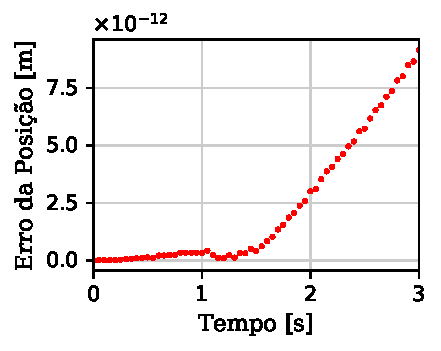
\includegraphics[scale=1]{images/falling_sphere/correct_initial_acceleration/position_error.pdf}
			\caption{}
			\label{subfig:position_error}
		\end{subfigure}
		\begin{subfigure}[t]{\smallresultsfigwidth}
			\centering
			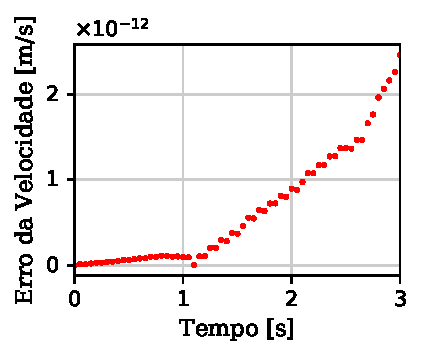
\includegraphics[scale=1]{images/falling_sphere/correct_initial_acceleration/velocity_error.pdf}
			\caption{}
			\label{subfig:velocity_error}
		\end{subfigure}
	}
	% \vspace{-0.2cm}
	\label{fig:falling_sphere_error}
	\sourceMe
	% \vspace{-1cm}
\end{figure}

Por sua vez, o erro da posição e o erro da velocidade, como funções do tempo, são apresentados na \cref{fig:falling_sphere_error}. Esses erros são calculados de acordo com a equação \eqref{eq:vector_error}. Observa-se nessa \namecref{fig:falling_sphere_error} que o erro da posição se mantém inferior a \SI{0,01}{\nano\meter} durante toda a simulação, evidenciando a exatidão do método. Além disso, é possível notar que o erro se acumula com o avanço da simulação.

O arquivo em formato \JSON{} utilizado para essa simulação é apresentado no \cref{app:code_listings}.

\section{Esfera Quicando}

Como extensão do problema de queda livre, o problema da esfera quicando inclui, além da gravidade, a colisão entre uma esfera e uma parede plana. Supõe-se uma partícula \(\particle\) esférica de raio \(\radius\) e massa \(\mass\) que, no instante inicial \(\initialInstant=0\), é liberada no espaço, em repouso, na posição \(\initial{\position} = \explicitVector{0}{\initial{\positiony}}{0}\).

A partícula está sujeita a um campo gravitacional constante cuja aceleração da gravidade é \(\gravity = -\gravityScalar\cdot\yUnit\) com \(\gravityScalar>0\). Nessa situação, a componente \(\positiony\) denota a altura da partícula.

Além disso, considera-se um elemento \(\element\) identificado com o plano \(\xAxis\zAxis\) representando o chão. Sendo um plano fixo, esse elemento é completamente determinado ao se fornecerem um ponto e um versor normal a ele. Para o plano \(\xAxis\zAxis\), podem ser adotados a origem \(\originPoint\) do sistema como ponto pertencente ao plano e o versor normal \(\planeNormalVersor = \explicitVector{0}{1}{0}\).

Essa configuração pode ser representada como na figura \ref{fig:bouncing_sphere}.

\begin{figure}[h]
	\caption{O problema da esfera quicando.}
	% \vspace{-0.5cm}
	\centering
		\alert{Colocar imagem representando o problema da esfera quicando}
		% 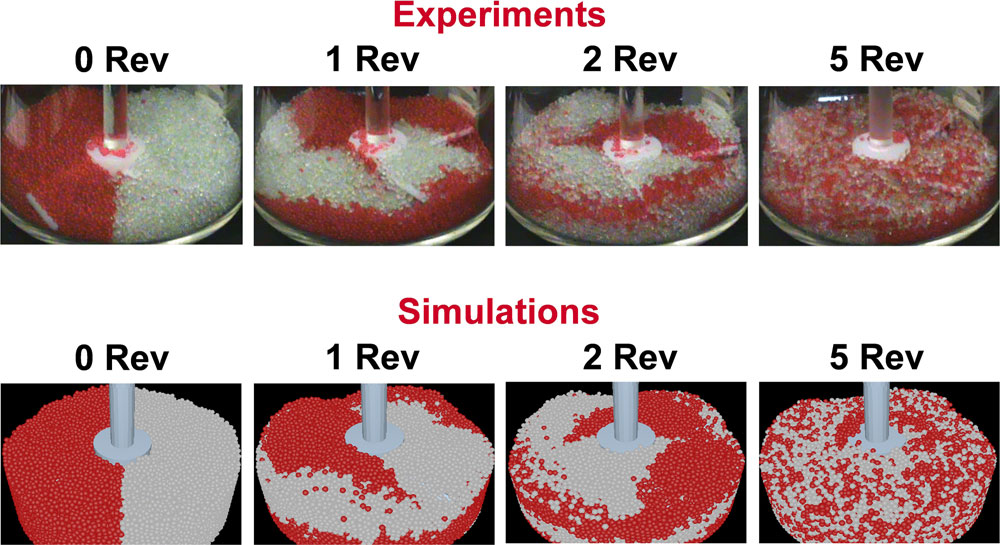
\includegraphics[width=0.65\textwidth]{images/drug_production.png}
	% {\centerline{\includegraphics[scale=#2]{#1}}}
	% \vspace{-0.2cm}
	\label{fig:bouncing_sphere}
	\source{\alert{Citar fonte}}
	% \vspace{-1cm}
\end{figure}

Além de servir como mais um caso para a validação do código, o problema da esfera quicando possibilita a comparação entre o coeficiente de restituição calculado a partir dos resultados da simulação e o coeficiente calculado analiticamente a partir do modelo de força escolhido.

A configuração do problema implica que a velocidade da esfera relativa ao plano é a sua própria velocidade vertical, já que o plano não se movimenta. Como consequência das equações \eqref{eq:antisymmetry_relative_velocity} e \eqref{eq:sphere_plane_relative_velocity}, essa velocidade é a própria velocidade da partícula.

Com isso, sendo \(\coefficientOfRestitution\) o coeficiente de restituição associado ao modelo de força de colisão escolhido, é possível mostrar que
\begin{equation} \label{eq:coefficient_of_restitution_with_gravity}
	\coefficientOfRestitution = - \dfrac{\afterCollision{\yComponent{\velocityScalar}} + \gravityScalar\cdot\collisionDuration}{\beforeCollision{\yComponent{\velocityScalar}}},
\end{equation}
sendo \(\afterCollision{\yComponent{\velocityScalar}}\) a velocidade da partícula \(\particle\) após a colisão com o chão, e \(\collisionDuration\), o tempo em que os corpos permanecem em contato. O termo \(\gravityScalar\cdot\collisionDuration\) é uma compensação feita pelo fato de que, no problema em questão, a gravidade contribui para a variação da velocidade das partículas, o que não é considerado no cálculo analítico do coeficiente de restituição.

Para a solução desse problema, foram escolhidos dois casos: um dissipativo (\cref{sec:results:bouncing_sphere:dissipative_case}), em que os elementos da simulação possuem constante de amortecimento não nula, e um conservativo (\cref{sec:results:bouncing_sphere:conservative}), em que essa constante é zero.

\subsection{Caso Dissipativo} \label{sec:results:bouncing_sphere:dissipative_case}

Para o estudo do problema da esfera quicando, foram considerados os parâmetros de simulação expostos na tabela \ref{tab:bouncing_sphere:dissipative_case:parameters}. O modelo de interação considerado é o modelo do amortecimento linear corrigido, cuja expressão para a força é dada pela \cref{eq:corrected_linear_dashpot:normal_force}, enquanto o coeficiente de restituição é calculado pela \cref{eq:corrected_linear_dashpot:coefficient_of_restitution}.

\begin{table}[h]
\centering
\caption{Parâmetros para o caso dissipativo do problema da esfera quicando.}
\label{tab:bouncing_sphere:dissipative_case:parameters}
\begin{parametersdesc}
	\item{Modelo de força normal}{\text{Amortecedor linear corrigido}}{\emptyUnit}
	\item{Gravidade}{\gravityScalar = 9,81}{\si[per-mode=symbol]{\metre\per\square\second}}
	\arrayrulecolor[gray]{0.8}\hline
	\item{Massa da partícula}{\ind{\mass}{\particle} = 1}{\si\kilogram}
	\item{Raio da partícula}{\ind{\radius}{\particle} = 3}{\si\centi\metre}
	\item{Constante elástica da partícula}{\ind{\elasticModulus}{\particle} = 1}{\si[per-mode=symbol]{\giga\pascal}}
	\item{Constante de amortecimento da partícula}{\ind{\normalDampingConstant}{\particle} = \SI{5000}{}}{\si[per-mode=symbol]{\newton\second\per\meter}}
	\arrayrulecolor[gray]{0.8}\hline
	\item{Altura inicial da partícula}{\initial{\positiony} = 1}{\si{\metre}}
	\item{Velocidade inicial da partícula}{\explicitVector{\initial{\velocityx}}{\initial{\velocityy}}{\initial{\velocityz}} = \explicitVector{0}{0}{0}}{\si[per-mode=symbol]{\metre\per\second}}
	\item{Aceleração inicial da partícula}{\explicitVector{\initial{\accelerationx}}{\initial{\accelerationy}}{\initial{\accelerationz}} = \explicitVector{0}{0}{0}}{\si[per-mode=symbol]{\metre\per\square\second}}
	\arrayrulecolor[gray]{0.8}\hline
	\item{Ponto da parede}{\ind{\planeOrigin}{\element} = \explicitVector{0}{0}{0}}{\si\meter}
	\item{Versor normal à parede}{\ind{\planeNormalVersor}{\element} = \explicitVector{0}{1}{0}}{\si\metre}
	\item{Constante elástica da parede}{\ind{\elasticModulus}{\element} = 1}{\si[per-mode=symbol]{\giga\pascal}}
	\item{Constante de amortecimento da parede}{\ind{\normalDampingConstant}{\element} = \SI{5000}{}}{\si[per-mode=symbol]{\newton\second\per\meter}}
	\arrayrulecolor[gray]{0.8}\hline
	\item{Instante final}{\finalInstant = 10}{\si\second} 
	\item{Passo de tempo}{\Dt = 10^{-5}}{\si\second}
	\item{Ordem de extrapolação}{\taylorOrder = 7}{\emptyUnit}
	\arrayrulecolor{black}
\end{parametersdesc}
\sourceMe 
\end{table}

\begin{figure}[htb!]
	\caption{Solução para a altura da partícula no caso dissipativo do problema da esfera quicando.}
	\centering
		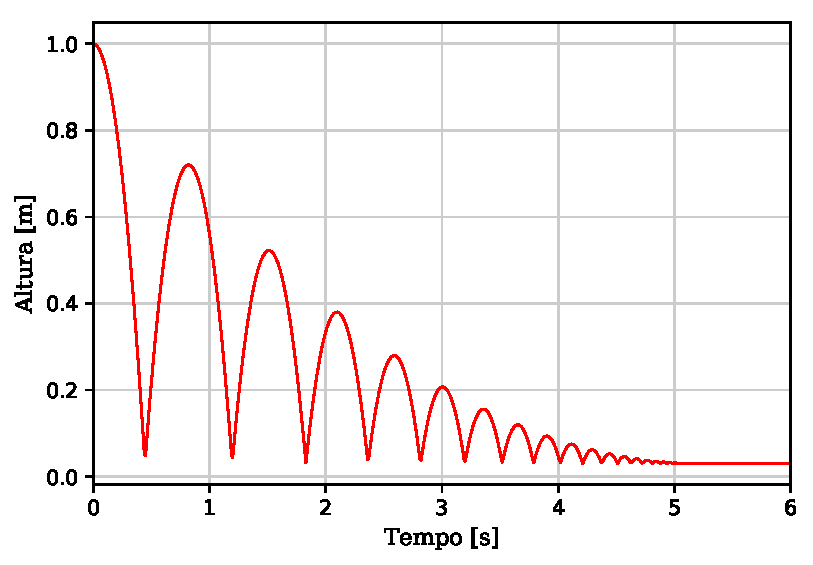
\includegraphics[scale=1]{images/bouncing_sphere/dissipative/y_position.pdf}
	\label{fig:bouncing_sphere_y_position}
	\sourceMe
\end{figure}

A partir desses parâmetros, uma simulação foi executada, resultando na altura da partícula em função do tempo como exposta na \cref{fig:bouncing_sphere_y_position}.

\begin{figure}[h]
	\caption[Energia cinética e energia mecânica da partícula no caso dissipativo do problema da esfera quicando.]{Energia cinética (\subref{subfig:bouncing_sphere:kinetic_energy}) e energia mecânica (\subref{subfig:bouncing_sphere:mechanical_energy}) da partícula no caso dissipativo do problema da esfera quicando.}
	% \vspace{-0.5cm}
	\centering
	\captionsetup[subfloat]{labelfont=bf}
	\subfloat{
		\centering
		\begin{subfigure}[t]{\smallresultsfigwidth}
			\centering
			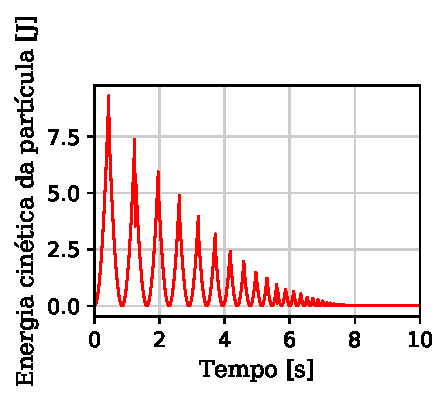
\includegraphics[scale=1]{images/bouncing_sphere/dissipative/kinetic_energy.pdf}
			\caption{}
			\label{subfig:bouncing_sphere:kinetic_energy}
		\end{subfigure}
		\begin{subfigure}[t]{\smallresultsfigwidth}
			\centering
			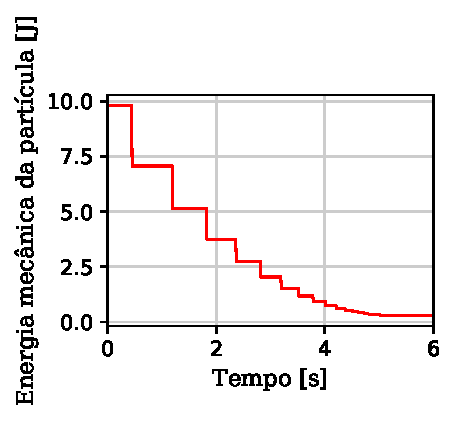
\includegraphics[scale=1]{images/bouncing_sphere/dissipative/mechanical_energy.pdf}
			\caption{}
			\label{subfig:bouncing_sphere:mechanical_energy}
		\end{subfigure}
	}
	\sourceMe
	\label{fig:bouncing_sphere_energy}
	% \vspace{-1cm}
\end{figure}

Uma análise importante a se fazer nesse problema é a da energia. A energia cinética e a energia mecânica resultantes da simulação, calculadas de acordo com as \cref{eq:kineticEnergy,eq:mechanicalEnergy}, são apresentadas na \cref{fig:bouncing_sphere_energy}. Observa-se nos gráficos que a partícula experiencia uma queda em sua sua energia mecânica após as colisões com o chão, sendo que a energia cinética anula-se aproximadamente após \SI{5}{\second} de simulação.

\begin{figure}[h]
	\caption{Coeficiente de restituição resultante da colisão dissipativa do problema da esfera quicando.}
	% \vspace{-0.5cm}
	\centering
		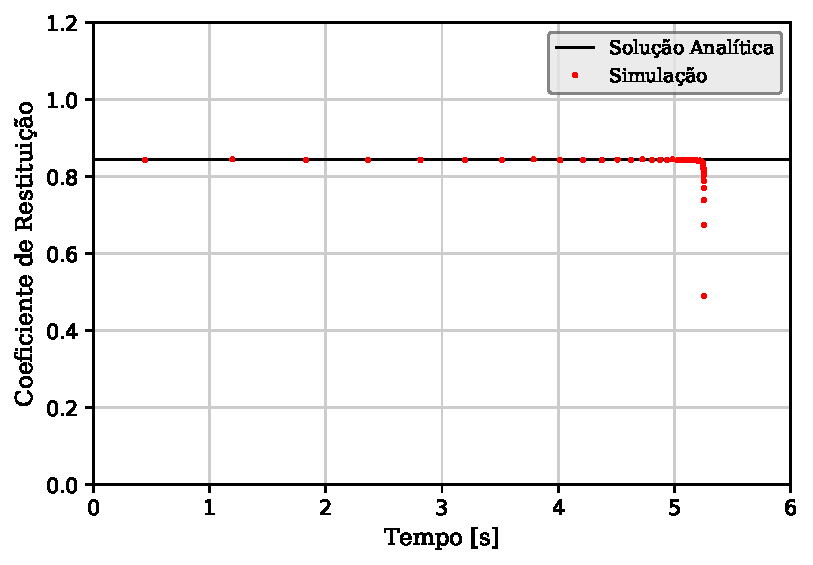
\includegraphics[scale=1]{images/bouncing_sphere/dissipative/coefficient_of_restitution.pdf}
		% 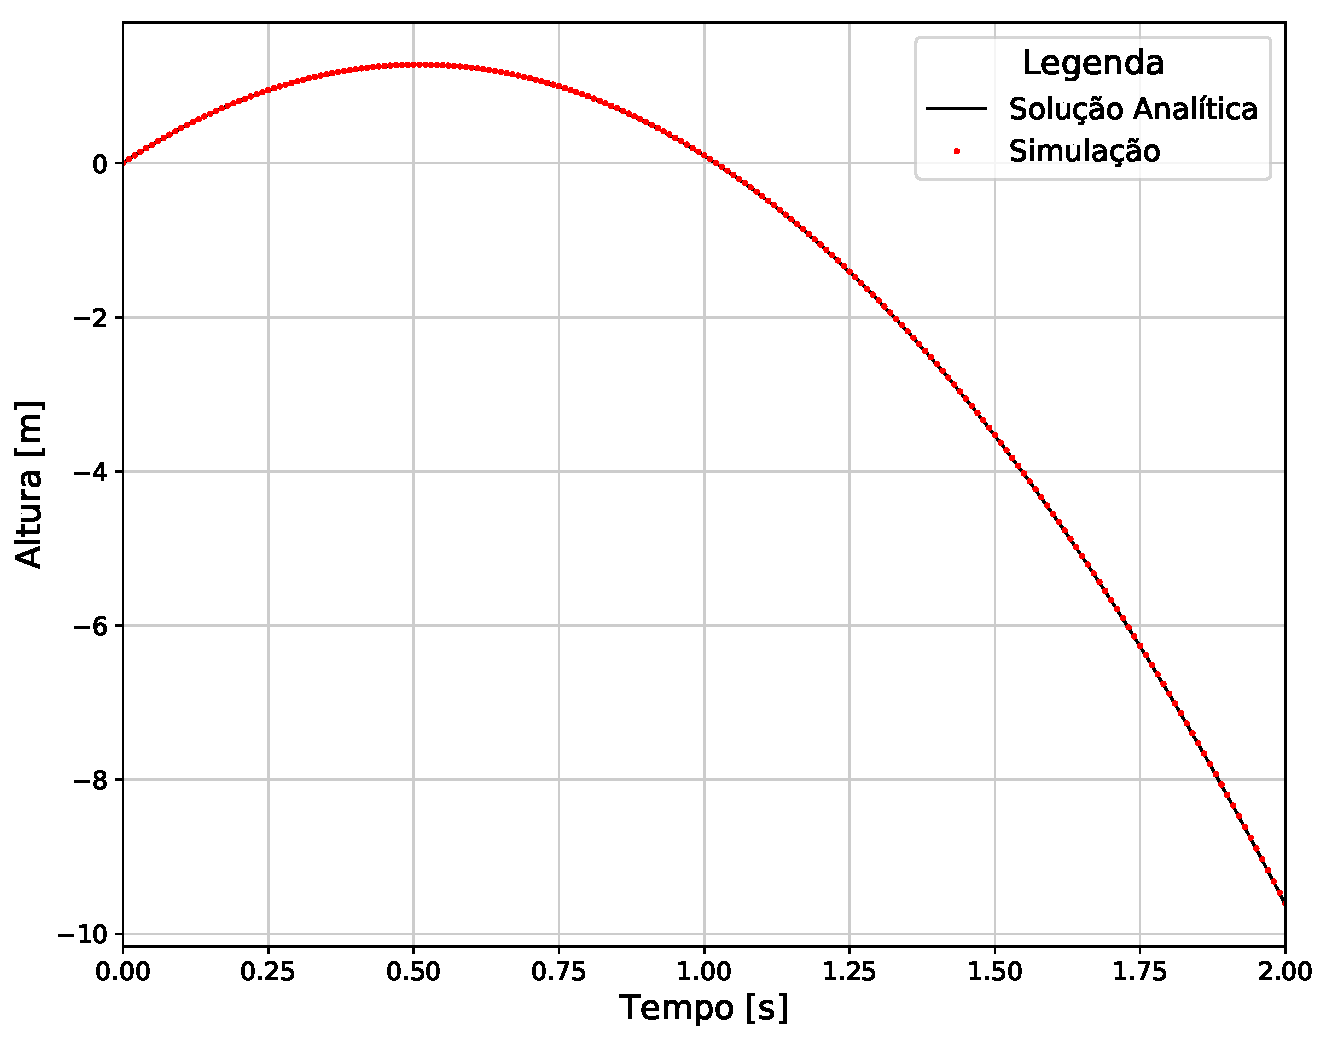
\includegraphics[width=\normalresultsfigwidth]{images/falling_sphere/y_position.pdf}
	% {\centerline{\includegraphics[scale=#2]{#1}}}
	% \vspace{-0.2cm}
	\label{fig:bouncing_sphere:dissipative:coefficient_of_restitution}
	\sourceMe
	% \vspace{-1cm}
\end{figure}

Além da energia, o coeficiente de restituição resultante da colisão também pode ser estudado. Na \cref{fig:bouncing_sphere:dissipative:coefficient_of_restitution}, estão representados o coeficiente calculado numericamente através da \cref{eq:coefficient_of_restitution_with_gravity} e o coeficiente analítico dado pela expressão \eqref{eq:corrected_linear_dashpot:coefficient_of_restitution}. Observa-se uma boa concordância entre os resultados até aproximadamente \SI{5}{\second} de simulação. A divergência que ocorre após esse instante explica-se pelo fato de que a partícula entra em repouso sobre o chão.

\subsection{Caso Conservativo} \label{sec:results:bouncing_sphere:conservative}

O caso dissipativo, como exposto na \cref{sec:results:bouncing_sphere:dissipative_case}, apresenta uma dissipação da energia causada pelo amortecimento do modelo de colisão adotado. Nesta \namecref{sec:results:bouncing_sphere:conservative}, considera-se o caso conservativo.

\begin{table}[h]
\centering
\caption{Parâmetros para o caso dissipativo do problema da esfera quicando.}
\label{tab:bouncing_sphere:conservative:parameters}
\begin{parametersdesc}
	\item{Constante de amortecimento da partícula}{\ind{\normalDampingConstant}{\particle} = 0}{\si[per-mode=symbol]{\newton\second\per\meter}}
	\item{Constante de amortecimento da paOrede}{\ind{\normalDampingConstant}{\element} = 0}{\si[per-mode=symbol]{\newton\second\per\meter}}
	\item{Demais parâmetros}{\text{\Cref{tab:bouncing_sphere:dissipative_case:parameters}}}{}
\end{parametersdesc}
\sourceMe 
\end{table}
\alert{Essa tabela ficou feia!}

\alert{Tirar o gráfico da energia e dizer que ela se conserva exceto nos choques}

\begin{figure}[htb!]
	\caption[Altura e energia mecânica da partícula e coeficiente de restituição no caso conservativo do problema da esfera quicando.]{Altura (\subref{subfig:bouncing_sphere:conservative:height}) e energia mecânica (\subref{subfig:bouncing_sphere:conservative:mechanical_energy}) da partícula e coeficiente de restituição (\subref{subfig:bouncing_sphere:conservative:coefficient_of_restitution}) no caso conservativo do problema da esfera quicando.}
	\centering
	\captionsetup[subfloat]{labelfont=bf}
	\subfloat{
		\centering
		\begin{subfigure}[t]{\smallresultsfigwidth}
			\centering
			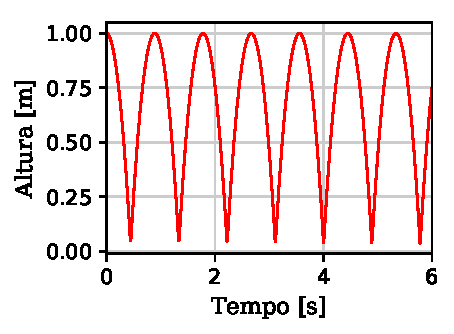
\includegraphics[scale=1]{images/bouncing_sphere/conservative/small_y_position.pdf}
			\caption{}
			\label{subfig:bouncing_sphere:conservative:height}
		\end{subfigure}
		\begin{subfigure}[t]{\smallresultsfigwidth}
			\centering
			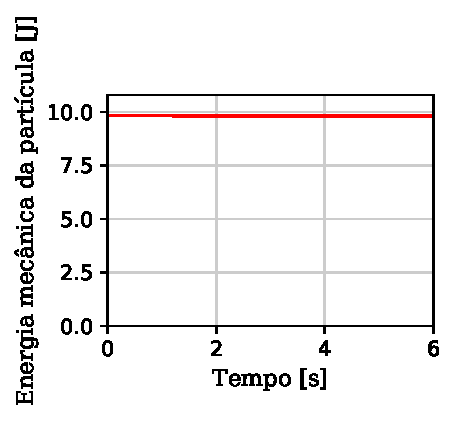
\includegraphics[scale=1]{images/bouncing_sphere/conservative/mechanical_energy.pdf}
			\caption{}
			\label{subfig:bouncing_sphere:conservative:mechanical_energy}
		\end{subfigure}
		\begin{subfigure}[t]{\smallresultsfigwidth}
			\centering
			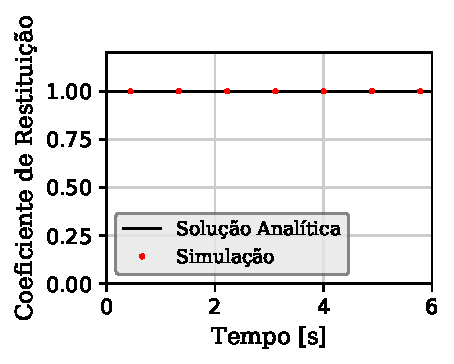
\includegraphics[scale=1]{images/bouncing_sphere/conservative/small_coefficient_of_restitution.pdf}
			\caption{}
			\label{subfig:bouncing_sphere:conservative:coefficient_of_restitution}
		\end{subfigure}
	}
	\sourceMe
	\label{fig:bouncing_sphere:conservative}
\end{figure}

Para essa simulação, foram utilizados parâmetros idênticos aos indicados na \cref{tab:bouncing_sphere:dissipative_case:parameters}, à exceção das constantes de amortecimento. Essas constantes são responsáveis pela dissipação da energia, e, para o caso conservativo, devem tomar valor nulo, como indicado na \cref{tab:bouncing_sphere:conservative:parameters}.

\begin{table}[h]
\centering
\caption{Energia mecânica e coeficiente de restituição resultantes do caso conservativo do problema da esfera quicando.}
\label{tab:bouncing_sphere:conservative:energy_and_coefficient_of_restitution}
\begin{parametersdesc}
	\item{Energia mecânica inicial}{\initial{\mechanicalEnergy} = \SI{9,81}{\joule}}{}
	\item{Energia mecânica final}{\final{\mechanicalEnergy} = \SI{9,80644775955}{\joule}}{}
	\item{Variação da energia mecânica}{\Delta \mechanicalEnergy = \initial{\mechanicalEnergy} - \final{\mechanicalEnergy} = \SI{3,552}{\milli\joule}}{}
	\item{Percentual de energia dissipada}{\bigslant{\Delta\mechanicalEnergy}{\initial{\mechanicalEnergy}} = \SI{0,036}{\percent}}{}
	\item{Coeficiente de restituição analítico}{\coefficientOfRestitution = 1}{}
	\item{Erro máximo do coeficiente de restituição}{\maximumErrorOf{\coefficientOfRestitution} = 2\cdot 10^{-4}}{}
	\item{Erro máximo percentual do coeficiente de restituição}{\bigslant{\maximumErrorOf{\coefficientOfRestitution}}{\coefficientOfRestitution} = \SI{0,02}{\percent}}{}
\end{parametersdesc}
\sourceMe 
\end{table}

Nessa situação, os resultados obtidos pela simulação para a altura e a energia mecânica da partícula e para o coeficiente de restituição são obtidos como na \cref{fig:bouncing_sphere:conservative}. Observa-se nessa \namecref{fig:bouncing_sphere:conservative} que a energia se conserva, sendo constante com exceção dos instantes de colisão, em que a energia mecânica se transforma em energia puramente elástica. De fato, a diferença observada entre a energia mecânica inicial \(\initial{\mechanical{\energy}}\) e a final \(\final{\mechanical{\energy}}\) foi da ordem de \(10^{-3}\si{\joule}\), o que representa \SI{0,036}{\percent} da energia inicial. Por sua vez, o coeficiente de restituição manteve-se bastante próximo de \(1\), o que corresponde ao resultado analítico, com erro máximo de \SI{0,02}{\percent}. Esses resultados estão expostos na \cref{tab:bouncing_sphere:conservative:energy_and_coefficient_of_restitution}.


\section{Colisão entre Esferas} \label{sec:results:colliding_spheres}

A questão central dos métodos de elementos discretos é a interação entre partículas, situação em que existem duas ou mais equações de movimento a serem resolvidas simultaneamente. Nesta \namecref{sec:results:colliding_spheres}, é apresentado o problema da colisão entre duas esferas.

\begin{figure}[h]
	\caption{O problema da colisão entre esferas.}
	% \vspace{-0.5cm}
	\centering
		\alert{Colocar imagem representando o problema da colisão entre esferas}
		% 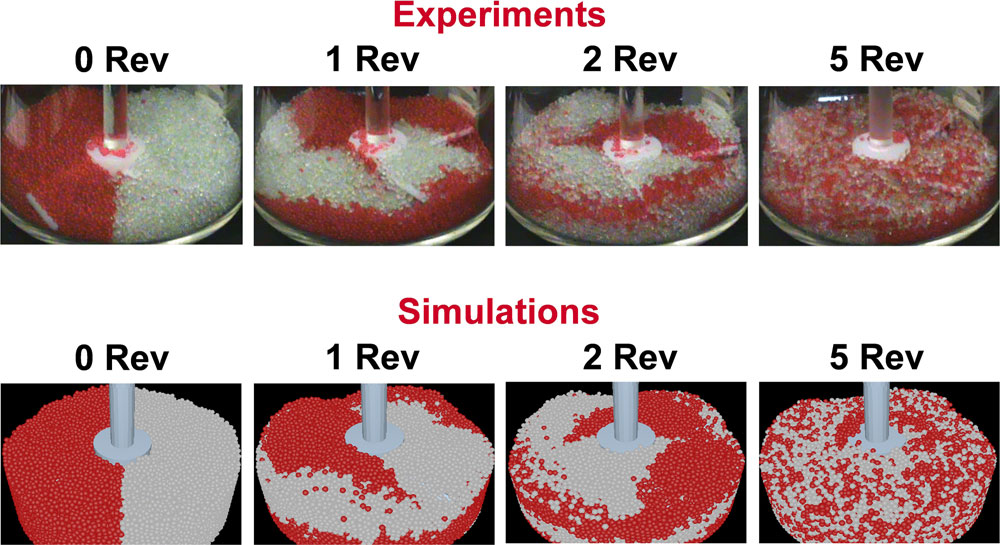
\includegraphics[width=0.65\textwidth]{images/drug_production.png}
	% {\centerline{\includegraphics[scale=#2]{#1}}}
	% \vspace{-0.2cm}
	\label{fig:colliding_spheres}
	\source{\alert{Citar fonte}}
	% \vspace{-1cm}
\end{figure}

Consideram-se duas partículas esféricas: a partícula vermelha \(\redParticle\) e a azul \(\blueParticle\). A partícula azul encontra-se em repouso na posição \(\initial{\bluePosition}\). A partícula vermelha encontra-se inicialmente na posição \(\initial{\redPosition}\) e avança, com uma velocidade linear \(\initial{\redVelocity}\) e uma velocidade angular \(\initial{\redAngularVelocity} = \initial{\redAngularVelocityScalar}\cdot\zUnit\), na direção de \(\blueParticle\). As partículas colidem, e ocorre transferência de movimento da partícula vermelha para a azul. Essa situação é representada na \cref{fig:colliding_spheres}.

Nesse problema, não é considerada a ação da gravidade, o que permite a análise simples das quantidades de movimento linear a angular. Como no problema da esfera quicando, são consideradas duas situações: o caso conservativo e o caso dissipativo. Devido à natureza das forças tangenciais apresentadas na \cref{sec:collision_force_models}, simulações com rotações são intrinsecamente dissipativas, e por isso esse caso só é considerado na \cref{sec:colliding_spheres:dissipative}.

\subsection{Caso Conservativo}

Para a simulação com conservação da energia, foram escolhidos os parâmetros expostos na \cref{tab:colliding_spheres:conservative:parameters}. Novamente, foi escolhido o modelo de força normal de amortecimento linear pela facilidade de se examinar o coeficiente de restituição resultante.

\begin{table}[h]
\centering
\caption{Parâmetros para o caso conservativo do problema da esfera quicando.}
\label{tab:colliding_spheres:conservative:parameters}
\begin{parametersdesc}
	\item{Modelo de força normal}{\text{Amortecedor linear corrigido}}{\emptyUnit}
	\arrayrulecolor[gray]{0.8}\hline
	\item{Massa da partícula vermelha}{\redMass = 1}{\si\kilogram}
	\item{Raio da partícula vermelha}{\redRadius = 3}{\si\centi\metre}
	\item{Constante elástica da partícula vermelha}{\redElasticModulus = 1}{\si[per-mode=symbol]{\giga\pascal}}
	\item{Constante de amortecimento normal da partícula vermelha}{\redNormalDampingConstant = 0}{\si[per-mode=symbol]{\newton\second\per\meter}}
	\arrayrulecolor[gray]{0.8}\hline
	\item{Posição inicial da partícula vermelha}{\initial{\redPosition} = \explicitVector{0}{0}{0}}{\si{\metre}}
	\item{Velocidade inicial da partícula vermelha}{\initial{\redVelocity} = \explicitVector{10}{0}{0}}{\si[per-mode=symbol]{\metre\per\second}}
	\item{Aceleração inicial da partícula vermelha}{\initial{\redAcceleration} = \explicitVector{0}{0}{0}}{\si[per-mode=symbol]{\metre\per\square\second}}
	\arrayrulecolor[gray]{0.8}\hline
	\item{Massa da partícula azul}{\blueMass = 1}{\si\kilogram}
	\item{Raio da partícula azul}{\blueRadius = 3}{\si\centi\metre}
	\item{Constante elástica da partícula azul}{\blueElasticModulus = 1}{\si[per-mode=symbol]{\giga\pascal}}
	\item{Constante de amortecimento normal da partícula azul}{\blueNormalDampingConstant = 0}{\si[per-mode=symbol]{\newton\second\per\meter}}
	\arrayrulecolor[gray]{0.8}\hline
	\item{Posição inicial da partícula azul}{\initial{\bluePosition} = \explicitVector{62}{0}{0}}{\si{\milli\metre}}
	\item{Velocidade inicial da partícula azul}{\initial{\blueVelocity} = \explicitVector{0}{0}{0}}{\si[per-mode=symbol]{\metre\per\second}}
	\item{Aceleração inicial da partícula azul}{\initial{\blueAcceleration} = \explicitVector{0}{0}{0}}{\si[per-mode=symbol]{\metre\per\square\second}}
	\arrayrulecolor[gray]{0.8}\hline
	\item{Instante final}{\finalInstant = 1}{\si\milli\second} 
	\item{Passo de tempo}{\Dt = 10^{-8}}{\si\second}
	\item{Ordem de extrapolação}{\taylorOrder = 7}{\emptyUnit}
	\arrayrulecolor{black}
\end{parametersdesc}
\sourceMe 
\end{table}

Com esses parâmetros, foi executada a simulação conservativa. A posição e a velocidade das partículas são apresentadas na \cref{fig:colliding_spheres:conservative:position_and_velocity}.

\begin{figure}[htb!]
	\caption[Solução para a posição horizontal e a velocidade horizontal das partículas colidentes na simulação conservativa.]{Solução para a posição horizontal (\subref{subfig:colliding_spheres:conservative:x_position}) e a velocidade horizontal (\subref{subfig:colliding_spheres:conservative:x_velocity}) das partículas colidentes na simulação conservativa.}
	\centering
	\captionsetup[subfloat]{labelfont=bf}
	\subfloat{
		\centering
		\begin{subfigure}[t]{\smallresultsfigwidth}
			\centering
			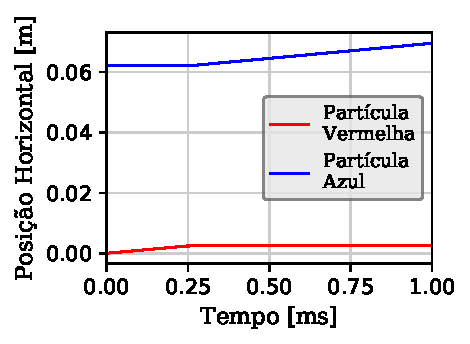
\includegraphics[scale=1]{images/colliding_spheres/conservative/Position-X_small.pdf}
			\caption{}
			\label{subfig:colliding_spheres:conservative:x_position}
		\end{subfigure}
		\begin{subfigure}[t]{\smallresultsfigwidth}
			\centering
			\includegraphics[scale=1]{images/colliding_spheres/conservative/Velocity-X_small.pdf}
			\caption{}
			\label{subfig:colliding_spheres:conservative:x_velocity}
		\end{subfigure}
	}
	\label{fig:colliding_spheres:conservative:position_and_velocity}
	\sourceMe
\end{figure}

Também é possível representarem-se a quantidade de movimento linear horizontal, a força de contato horizontal entre as partículas, a energia cinética e o coeficiente de restituição resultante do choque, como na \cref{fig:colliding_spheres:conservative:linear_momentum_force_kinetic_energy_and_coefficient_of_restitution}.

\begin{figure}[htb!]
	\caption[Curvas da quantidade de movimento linear, da força de contato horizontal, da energia cinética e do coeficiente de restituição do par de partículas colidentes na simulação conservativa.]{Curvas da quantidade de movimento linear (\subref{subfig:colliding_spheres:conservative:x_linear_momentum}), da força de contato horizontal (\subref{subfig:colliding_spheres:conservative:x_contact_force}), da energia cinética (\subref{subfig:colliding_spheres:conservative:kinetic_energy}) e do coeficiente de restituição (\subref{subfig:colliding_spheres:conservative:coefficient_of_restitution}) do par de partículas colidentes na simulação conservativa.}
	\centering
	\captionsetup[subfloat]{labelfont=bf}
	\subfloat{
		\centering
		\begin{subfigure}[t]{\smallresultsfigwidth}
			\centering
			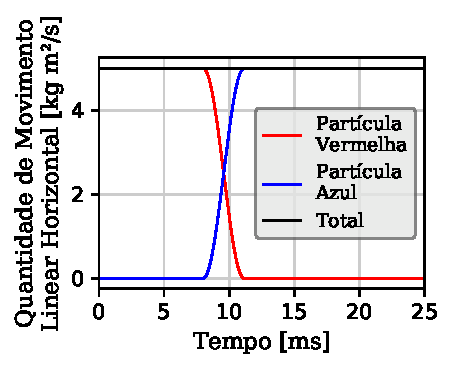
\includegraphics[scale=1]{images/colliding_spheres/conservative/linearMomentum-X_small_total.pdf}
			\caption{}
			\label{subfig:colliding_spheres:conservative:x_linear_momentum}
		\end{subfigure}
		\begin{subfigure}[t]{\smallresultsfigwidth}
			\centering
			\includegraphics[scale=1]{images/colliding_spheres/conservative/contactForce-X_small.pdf}
			\caption{}
			\label{subfig:colliding_spheres:conservative:x_contact_force}
		\end{subfigure}
		\begin{subfigure}[t]{\smallresultsfigwidth}
			\centering
			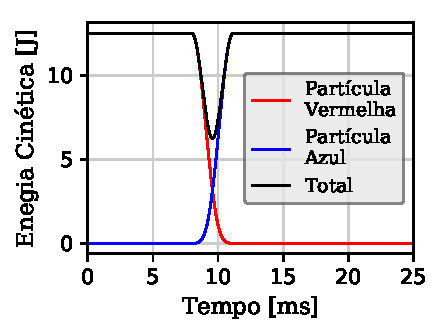
\includegraphics[scale=1]{images/colliding_spheres/conservative/kineticEnergy_small_total.pdf}
			\caption{}
			\label{subfig:colliding_spheres:conservative:kinetic_energy}
		\end{subfigure}
		\begin{subfigure}[t]{\smallresultsfigwidth}
			\centering
			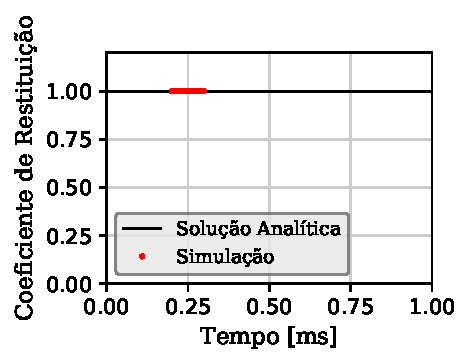
\includegraphics[scale=1]{images/colliding_spheres/conservative/coefficient_of_restitution_small.pdf}
			\caption{}
			\label{subfig:colliding_spheres:conservative:coefficient_of_restitution}
		\end{subfigure}
	}
	\label{fig:colliding_spheres:conservative:linear_momentum_force_kinetic_energy_and_coefficient_of_restitution}
	\sourceMe
\end{figure}

\begin{table}[h]
\centering
\caption{Coeficiente de restituição resultante do caso conservativo do problema das esferas colidentes.}
\label{tab:colliding_spheres:conservative:energy_and_coefficient_of_restitution}
\begin{parametersdesc}
	\item{Coeficiente de restituição analítico}{\coefficientOfRestitution = 1}{}
	\item{Erro máximo do coeficiente de restituição}{\maximumErrorOf{\coefficientOfRestitution} = 9\cdot 10^{-9}}{}
\end{parametersdesc}
\sourceMe 
\end{table}

Como pode ser observado, os resultados aproximam-se bastante do esperado. Por se tratar de uma colisão sem termos dissipativos, a partícula vermelha transfere todo o seu movimento à azul, entrando em repouso após a colisão. A \cref{subfig:colliding_spheres:conservative:coefficient_of_restitution} e a \cref{tab:colliding_spheres:conservative:energy_and_coefficient_of_restitution} indicam que o coeficiente de restituição numericamente calculado praticamente se iguala ao analítico com valor unitário, o que implica uma colisão perfeitamente elástica. Mais ainda, infere-se das \cref{subfig:colliding_spheres:conservative:x_linear_momentum,subfig:colliding_spheres:conservative:kinetic_energy} que ocorre a conservação da quantidade de movimento e a conservação da energia. Além disso, chama a atenção o fato de que parte da energia cinética é transformada em energia elástica durante o choque, e é restituída finda a colisão. Também é interessante notar que a força de colisão entre as partículas, indicada na \cref{subfig:colliding_spheres:conservative:x_contact_force}, ultrapassa os \SI{150}{\kilo\newton} em módulo.

\subsection{Caso Dissipativo} \label{sec:colliding_spheres:dissipative}

No caso dissipativo, são atribuídas às partículas constantes de amortecimento não nulas. A simulação dissipativa pode ser separada em dois casos: sem rotação e com rotação.

\subsubsection{Sem Rotação}

Para a simulação dissipativa sem rotação, consideram-se os parâmetros da \cref{tab:colliding_spheres:dissipative:parameters}. Os resultados desse caso podem ser compilados como na \cref{fig:colliding_spheres:dissipative:results}.

\begin{table}[h]
\centering
\caption{Parâmetros para o caso dissipativo do problema da colisão entre esferas.}
\label{tab:colliding_spheres:dissipative:parameters}
\begin{parametersdesc}
	\item{Constante de amortecimento da partícula vermelha}{\redNormalDampingConstant = 10000}{\si[per-mode=symbol]{\newton\second\per\meter}}
	\item{Constante de amortecimento da partícula azul}{\blueNormalDampingConstant = 10000}{\si[per-mode=symbol]{\newton\second\per\meter}}
	\item{Demais parâmetros}{\text{\Cref{tab:colliding_spheres:conservative:parameters}}}{}
\end{parametersdesc}
\sourceMe 
\end{table}

\begin{figure}[htb!]
	\caption[Solução da posição, da velocidade, da quantidade de movimento linear, da força de contato horizontal, da energia cinética e do coeficiente de restituição do par de partículas colidentes na simulação dissipativa sem rotação.]{Solução da posição (\subref{subfig:colliding_spheres:dissipative:x_position}), da velocidade (\subref{subfig:colliding_spheres:dissipative:x_velocity}), da quantidade de movimento linear (\subref{subfig:colliding_spheres:dissipative:x_linear_momentum}), da força de contato horizontal (\subref{subfig:colliding_spheres:dissipative:x_contact_force}), da energia cinética (\subref{subfig:colliding_spheres:dissipative:kinetic_energy}) e do coeficiente de restituição (\subref{subfig:colliding_spheres:dissipative:coefficient_of_restitution}) do par de partículas colidentes na simulação dissipativa sem rotação.}
	\vspace*{-0.5cm}
	\centering
	\captionsetup[subfloat]{labelfont=bf}
	\subfloat{
		\centering
		\begin{subfigure}[t]{\smallresultsfigwidth}
			\centering
			\includegraphics[scale=1]{images/colliding_spheres/dissipative/Position-X_small.pdf}
			\caption{}
			\label{subfig:colliding_spheres:dissipative:x_position}
		\end{subfigure}
		\begin{subfigure}[t]{\smallresultsfigwidth}
			\centering
			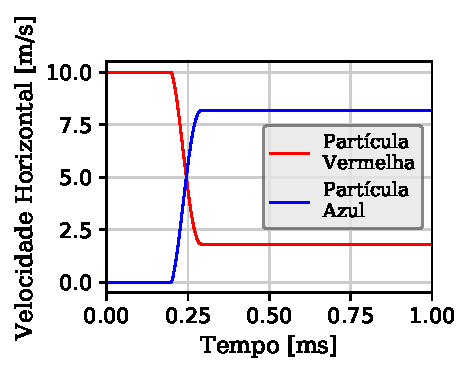
\includegraphics[scale=1]{images/colliding_spheres/dissipative/Velocity-X_small.pdf}
			\caption{}
			\label{subfig:colliding_spheres:dissipative:x_velocity}
		\end{subfigure}
		\begin{subfigure}[t]{\smallresultsfigwidth}
			\centering
			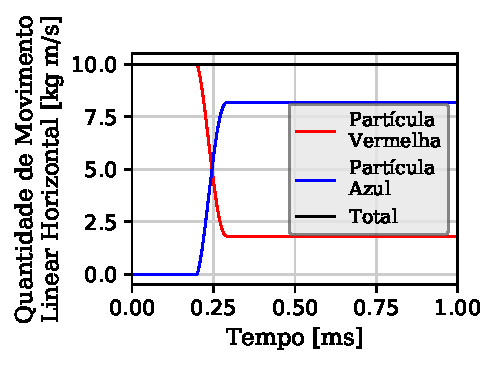
\includegraphics[scale=1]{images/colliding_spheres/dissipative/linearMomentum-X_small_total_alternative.pdf}
			\caption{}
			\label{subfig:colliding_spheres:dissipative:x_linear_momentum}
		\end{subfigure}
		\begin{subfigure}[t]{\smallresultsfigwidth}
			\centering
			\includegraphics[scale=1]{images/colliding_spheres/dissipative/contactForce-X_small.pdf}
			\caption{}
			\label{subfig:colliding_spheres:dissipative:x_contact_force}
		\end{subfigure}
		\begin{subfigure}[t]{\smallresultsfigwidth}
			\centering
			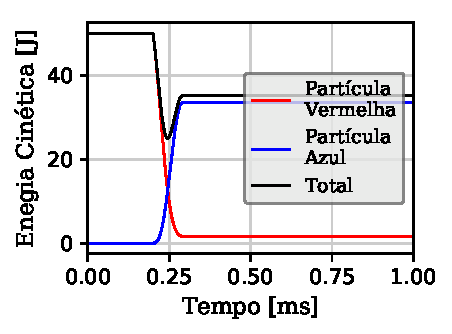
\includegraphics[scale=1]{images/colliding_spheres/dissipative/kineticEnergy_small_total_alternative.pdf}
			\caption{}
			\label{subfig:colliding_spheres:dissipative:kinetic_energy}
		\end{subfigure}
		\begin{subfigure}[t]{\smallresultsfigwidth}
			\centering
			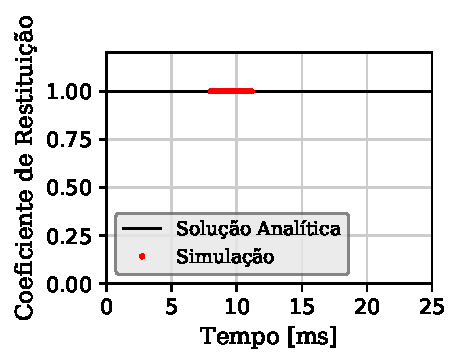
\includegraphics[scale=1]{images/colliding_spheres/dissipative/coefficient_of_restitution_small.pdf}
			\caption{}
			\label{subfig:colliding_spheres:dissipative:coefficient_of_restitution}
		\end{subfigure}
	}
	\label{fig:colliding_spheres:dissipative:results}
	\sourceMe
\end{figure}

Por fim, a simulação foi repetida com os parâmetros da \cref{tab:colliding_spheres:dissipative:parameters} à exceção do passo tempo, que foi variado. Foram executadas simulações para 
\begin{equation*}
	\Dt = 10^{-8},\quad{\sqrt{2}\cdot 10^{-8}},\quad{2\cdot 10^{-8}},\quad{2\sqrt{2}\cdot 10^{-8}},\quad{4\cdot 10^{-8}}, \dotsc, {1024\cdot 10^{-8}},
\end{equation*}
e o erro máximo do coeficiente de restituição foi computado. O resultado desse processo está exposto, em escala logarítmica, na \cref{fig:colliding_spheres:dissipative:coefficient_of_restitution_error}.

\begin{figure}[h]
	\caption{Erro máximo do coeficiente de restituição em função do passo de tempo no caso dissipativo do problema das esferas colidentes sem rotação.}
	\centering
	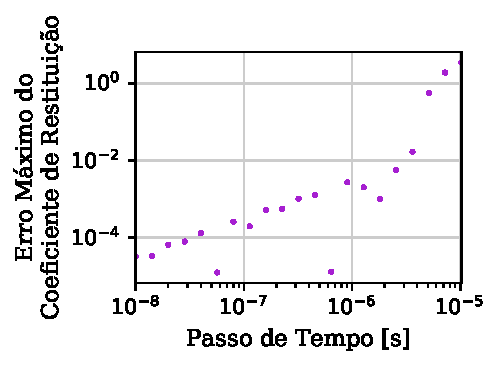
\includegraphics[scale=1]{images/colliding_spheres/dissipative/coefficient_of_restitution_error_loglog_small.pdf}
	\label{fig:colliding_spheres:dissipative:coefficient_of_restitution_error}
	\sourceMe
\end{figure}

Dentre as características que se observam nesses resultados, nota-se que a partícula vermelha, ao contrário do caso sem amortecimento, não entra em repouso após a colisão, mas, sim, continua a sua trajetória com uma velocidade reduzida. Também, a energia cinética total do sistema não se conserva, sofrendo uma queda de aproximadamente \SI{16,5}{\joule} do início até o fim da simulação. Embora ocorra a perda de energia, a quantidade de movimento linear mantém-se constante, como deve acontecer em qualquer sistema sem forças externas, mesmo que existam forças internas dissipativas. O coeficiente de restituição obtido foi de \SI{0,63}{}, apresentando um erro de apenas \(3,18\cdot 10^{-5}\) com relação ao coeficiente calculado analiticamente. Além dessas considerações, percebe-se, comparando-se as \cref{subfig:colliding_spheres:conservative:x_contact_force,subfig:colliding_spheres:dissipative:x_contact_force}, que ocorre uma alteração na curva da força de contato horizontal. No caso conservativo, existe uma simetria do gráfico com relação ao instante de máxima superposição, o que não se observa na força do caso dissipativo. Esse deslocamento no perfil de força, com intensidade maior na aproximação que no afastamento, é o responsável pela dissipação de energia. Por fim, observa-se que o erro máximo do coeficiente de restituição cresce com o aumento do passo de tempo, chegando a um erro de mais de \SI{100}{\percent} para passos de aproximadamente \(10^{-5}\si{\second}\).

\subsubsection{Com Rotação}

Para a colisão de partículas com rotação, utilizou-se o modelo de interação de Haff e Werner, que é o análogo rotacional do modelo do amortecedor linear, e cuja expressão para a força tangencial é dada pela \cref{eq:haff_werner}. Para a força normal, o modelo adotado ainda é o do amortecedor linear corrigido. Como entrada para a simulação, foram aplicados os parâmetros da \cref{tab:colliding_spheres:dissipative:rotation:parameters}. O momento de inércia das partículas é consequência de sua massa e seu raio, de acordo com a \cref{eq:momentOfInertia_for_spheres}.

\begin{table}[h]
\centering
\caption{Parâmetros para o caso dissipativo do problema da colisão entre esferas considerando rotações.}
\label{tab:colliding_spheres:dissipative:rotation:parameters}
\begin{parametersdesc}
	\item{Modelo de força normal}{\text{Amortecedor linear corrigido}}{\emptyUnit}
	\item{Modelo de força tangencial}{\text{Modelo de Haff e Werner}}{\emptyUnit}
	\arrayrulecolor[gray]{0.8}\hline
	\item{Momento de inércia da partícula vermelha}{\redMomentOfInertia = 3,6}{\si[per-mode=symbol]{\kilogram\square\centi\meter}}
	\item{Velocidade angular da partícula vermelha}{\initial{\redAngularVelocityScalar} = 100}{\si[per-mode=symbol]{\radian\per\second}}
	\item{Constante de amortecimento normal da partícula vermelha}{\redNormalDampingConstant = \SI{10000}{}}{\si[per-mode=symbol]{\newton\second\per\meter}}
	\item{Constante de amortecimento tangencial da partícula vermelha}{\redTangentialDampingConstant = \SI{10000}{}}{\si[per-mode=symbol]{\newton\second\per\meter}}
	\item{Coeficiente de atrito associado à partícula vermelha}{\redDynamicFriction = 0,95}{\emptyUnit}
	\arrayrulecolor[gray]{0.8}\hline
	\item{Momento de inércia da partícula azul}{\blueMomentOfInertia = 3,6}{\si[per-mode=symbol]{\kilogram\square\centi\meter}}
	\item{Constante de amortecimento normal da partícula azul}{\blueNormalDampingConstant = \SI{10000}{}}{\si[per-mode=symbol]{\newton\second\per\meter}}
	\item{Constante de amortecimento tangencial da partícula azul}{\blueTangentialDampingConstant = \SI{10000}{}}{\si[per-mode=symbol]{\newton\second\per\meter}}
	\item{Coeficiente de atrito associado à partícula azul}{\blueDynamicFriction = 0,95}{\emptyUnit}
	\arrayrulecolor[gray]{0.8}\hline
	\item{Demais parâmetros}{\text{\Cref{tab:colliding_spheres:conservative:parameters}}}{}
	\arrayrulecolor{black}
\end{parametersdesc}
\sourceMe 
\end{table}

Com esses parâmetros, foram obtidos os resultados expostos nas \cref{fig:colliding_spheres:dissipative_rotation:kinematic_results,fig:colliding_spheres:dissipative_rotation:momentum_results,fig:colliding_spheres:dissipative_rotation:forces_and_torque_results,fig:colliding_spheres:dissipative_rotation:energy_and_coefficient_of_restitution_results}. Observa-se, na \cref{fig:colliding_spheres:dissipative_rotation:kinematic_results}, que, na colisão, a rotação da partícula vermelha tem o efeito de iniciar um movimento na direção vertical. Ainda, em virtude da não elasticidade do choque, a partícula vermelha mantém-se em movimento mesmo após a colisão com a azul. Na \cref{fig:colliding_spheres:dissipative_rotation:momentum_results}, estão expostas as curvas da quantidade de movimento linear e da quantidade de movimento angular. Novamente, a simulação apresentou resultados fisicamente verossímeis, visto que ocorre a conservação dessas quantidades. 

Os gráficos da força e do torque sobre as partículas estão representados na \cref{fig:colliding_spheres:dissipative_rotation:forces_and_torque_results}. Nota-se que a força horizontal atinge a casa de \SI{100}{\kilo\newton}, enquanto a vertical alcança \SI{30}{\kilo\newton}. As partículas experienciam torques resultantes iguais em razão de serem, elas próprias, idênticas. 

Por sua vez, na \cref{fig:colliding_spheres:dissipative_rotation:energy_and_coefficient_of_restitution_results}, são expostas as curvas de energia e o coeficiente de restituição obtidos. Observa-se que, por conta da dissipação, todas as formas de energia sofrem redução. Devido ao modelo intrinsecamente dissipativo para a força tangencial, não existe energia rotacional armazenada elasticamente. A consequência disso é que não há recuperação da energia rotacional após a colisão, como vê na \cref{subfig:colliding_spheres:dissipative_rotation:rotational_energy}. 

Por fim, na \cref{subfig:colliding_spheres:dissipative_rotation:coefficient_of_restitution}, apresenta-se o coeficiente de restituição. Mais uma vez, observa-se a sua correspondência com o valor analítico. A \cref{tab:colliding_spheres:dissipative_rotation:energy_and_coefficient_of_restitution} sumariza os resultados para a energia cinética e o coeficiente de restituição.

\begin{table}[h]
\centering
\caption{Energia mecânica e coeficiente de restituição resultantes do caso conservativo do problema da esfera quicando.}
\label{tab:colliding_spheres:dissipative_rotation:energy_and_coefficient_of_restitution}
\begin{parametersdesc}
	\item{Energia mecânica inicial}{\initial{\mechanicalEnergy} = \SI{51,80}{\joule}}{}
	\item{Energia mecânica final}{\final{\mechanicalEnergy} = \SI{33,78}{\joule}}{}
	\item{Variação da energia mecânica}{\Delta \mechanicalEnergy = \initial{\mechanicalEnergy} - \final{\mechanicalEnergy} = \SI{18}{\joule}}{}
	\item{Percentual de energia dissipada}{\bigslant{\Delta\mechanicalEnergy}{\initial{\mechanicalEnergy}} = \SI{34,78}{\percent}}{}
	\item{Coeficiente de restituição analítico}{\coefficientOfRestitution = 0,64}{}
	\item{Erro máximo do coeficiente de restituição}{\maximumErrorOf{\coefficientOfRestitution} = 9,8\cdot 10^{-6}}{}
	\item{Erro máximo relativo do coeficiente de restituição}{\bigslant{\maximumErrorOf{\coefficientOfRestitution}}{\coefficientOfRestitution} = 1,5\cdot 10^{-6}}{}
\end{parametersdesc}
\sourceMe 
\end{table}

\begin{figure}[htb!]
	\caption[Solução das posições horizontal e vertical, das velocidades horizontal e vertical, e da velocidade angular das partículas no caso dissipativo do problema da colisão de esferas com rotação.]{Solução das posições horizontal (\subref{subfig:colliding_spheres:dissipative_rotation:x_position}) e vertical (\subref{subfig:colliding_spheres:dissipative_rotation:y_position}), das velocidades horizontal (\subref{subfig:colliding_spheres:dissipative_rotation:x_velocity}) e vertical (\subref{subfig:colliding_spheres:dissipative_rotation:y_velocity}), e da velocidade angular (\subref{subfig:colliding_spheres:dissipative_rotation:z_angular_velocity}) das partículas no caso dissipativo do problema da colisão de esferas com rotação.}
	\vspace*{-0.5cm}
	\centering
	\captionsetup[subfloat]{labelfont=bf}
	\subfloat{
		\centering
		\begin{subfigure}[t]{\smallresultsfigwidth}
			\centering
			\includegraphics[scale=1]{images/colliding_spheres/dissipative_rotation/Position-X_small.pdf}
			\caption{}
			\label{subfig:colliding_spheres:dissipative_rotation:x_position}
		\end{subfigure}
		\begin{subfigure}[t]{\smallresultsfigwidth}
			\centering
			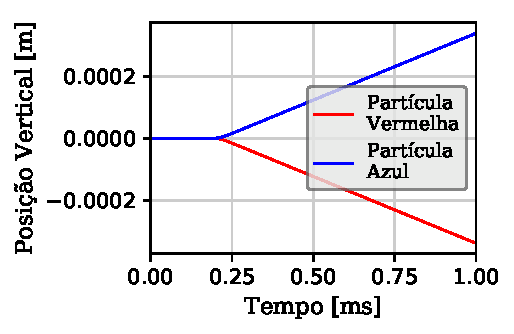
\includegraphics[scale=1]{images/colliding_spheres/dissipative_rotation/Position-Y_small.pdf}
			\caption{}
			\label{subfig:colliding_spheres:dissipative_rotation:y_position}
		\end{subfigure}
		\begin{subfigure}[t]{\smallresultsfigwidth}
			\centering
			\includegraphics[scale=1]{images/colliding_spheres/dissipative_rotation/Velocity-X_small.pdf}
			\caption{}
			\label{subfig:colliding_spheres:dissipative_rotation:x_velocity}
		\end{subfigure}
		\begin{subfigure}[t]{\smallresultsfigwidth}
			\centering
			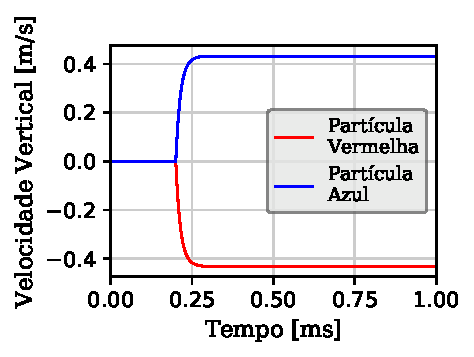
\includegraphics[scale=1]{images/colliding_spheres/dissipative_rotation/Velocity-Y_small.pdf}
			\caption{}
			\label{subfig:colliding_spheres:dissipative_rotation:y_velocity}
		\end{subfigure}
		\begin{subfigure}[t]{\smallresultsfigwidth}
			\centering
			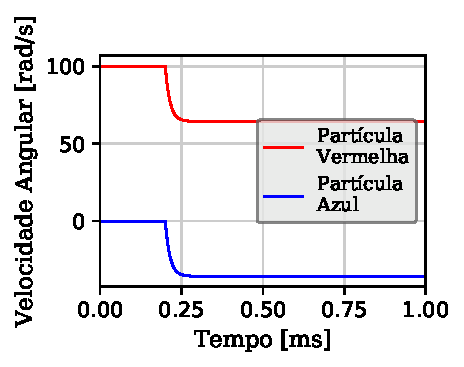
\includegraphics[scale=1]{images/colliding_spheres/dissipative_rotation/AngularVelocity-Z_small_alternative.pdf}
			\caption{}
			\label{subfig:colliding_spheres:dissipative_rotation:z_angular_velocity}
		\end{subfigure}
	}
	\label{fig:colliding_spheres:dissipative_rotation:kinematic_results}
	\sourceMe
\end{figure}

\begin{figure}[htb!]
	\caption[Solução numérica das quantidades de movimento linear horizontal, linear vertical e angular para o caso dissipativo do problema das esferas colidentes com rotação.]{Solução numérica das quantidades de movimento linear horizontal (\subref{subfig:colliding_spheres:dissipative_rotation:x_linear_momentum}), linear vertical (\subref{subfig:colliding_spheres:dissipative_rotation:y_linear_momentum}) e angular (\subref{subfig:colliding_spheres:dissipative_rotation:z_angular_momentum}) para o caso dissipativo do problema das esferas colidentes com rotação.}
	\vspace*{-0.5cm}
	\centering
	\captionsetup[subfloat]{labelfont=bf}
	\subfloat{
		\centering
		\begin{subfigure}[t]{\smallresultsfigwidth}
			\centering
			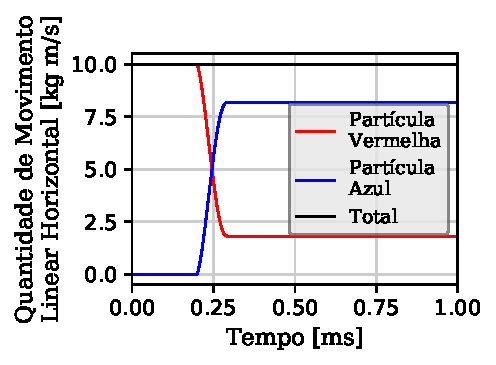
\includegraphics[scale=1]{images/colliding_spheres/dissipative_rotation/linearMomentum-X_small_total.pdf}
			\caption{}
			\label{subfig:colliding_spheres:dissipative_rotation:x_linear_momentum}
		\end{subfigure}
		\begin{subfigure}[t]{\smallresultsfigwidth}
			\centering
			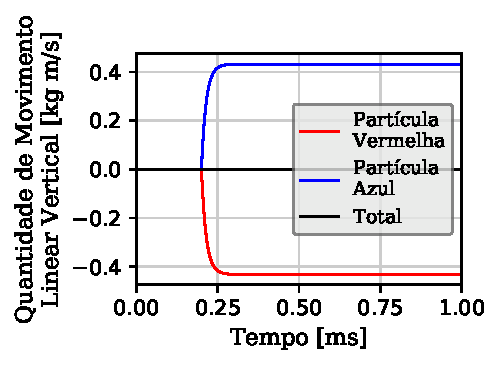
\includegraphics[scale=1]{images/colliding_spheres/dissipative_rotation/linearMomentum-Y_small_total.pdf}
			\caption{}
			\label{subfig:colliding_spheres:dissipative_rotation:y_linear_momentum}
		\end{subfigure}
		\begin{subfigure}[t]{\smallresultsfigwidth}
			\centering
			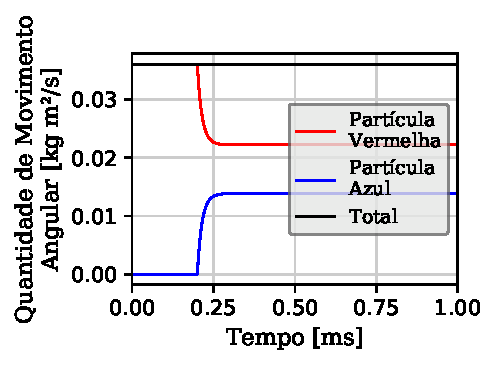
\includegraphics[scale=1]{images/colliding_spheres/dissipative_rotation/angularMomentum-Z_small_total_alternative.pdf}
			\caption{}
			\label{subfig:colliding_spheres:dissipative_rotation:z_angular_momentum}
		\end{subfigure}
	}
	\label{fig:colliding_spheres:dissipative_rotation:momentum_results}
	\sourceMe
\end{figure}

\begin{figure}[htb!]
	\caption[Forças horizontal e vertical e torque no caso dissipativo do problema das esferas colidentes com rotação.]{Forças horizontal (\subref{subfig:colliding_spheres:dissipative_rotation:x_contact_force}) e vertical (\subref{subfig:colliding_spheres:dissipative_rotation:y_contact_force}) e torque (\subref{subfig:colliding_spheres:dissipative_rotation:z_torque}) no caso dissipativo do problema das esferas colidentes com rotação.}
	\vspace*{-0.5cm}{}
	\centering
	\captionsetup[subfloat]{labelfont=bf}
	\subfloat{
		\centering
		\begin{subfigure}[t]{\smallresultsfigwidth}
			\centering
			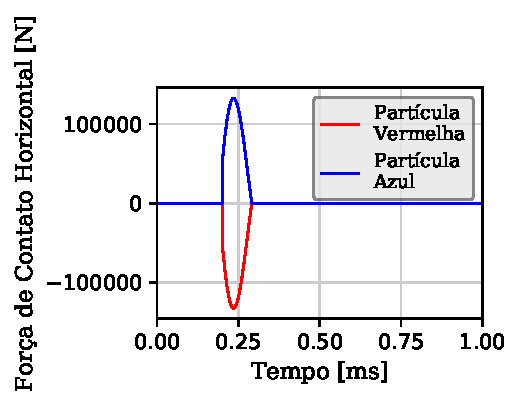
\includegraphics[scale=1]{images/colliding_spheres/dissipative_rotation/contactForce-X_small.pdf}
			\caption{}
			\label{subfig:colliding_spheres:dissipative_rotation:x_contact_force}
		\end{subfigure}
		\begin{subfigure}[t]{\smallresultsfigwidth}
			\centering
			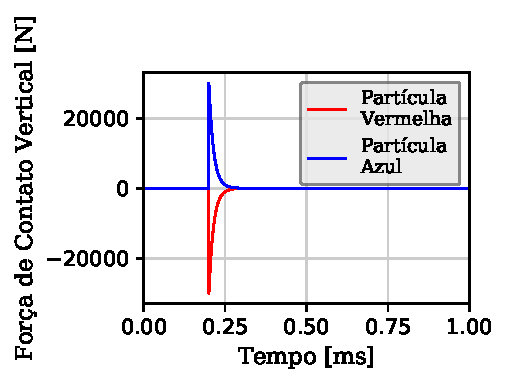
\includegraphics[scale=1]{images/colliding_spheres/dissipative_rotation/contactForce-Y_small.pdf}
			\caption{}
			\label{subfig:colliding_spheres:dissipative_rotation:y_contact_force}
		\end{subfigure}
		\begin{subfigure}[t]{\smallresultsfigwidth}
			\centering
			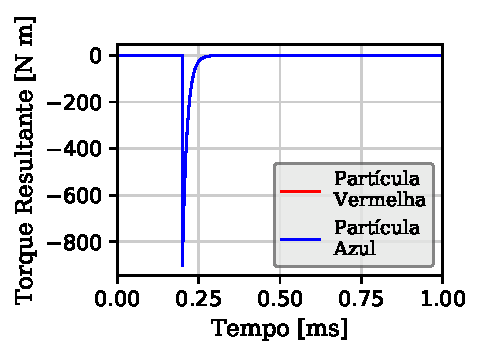
\includegraphics[scale=1]{images/colliding_spheres/dissipative_rotation/resultingTorque-Z_small.pdf}
			\caption{}
			\label{subfig:colliding_spheres:dissipative_rotation:z_torque}
		\end{subfigure}
	}
	\label{fig:colliding_spheres:dissipative_rotation:forces_and_torque_results}
	\sourceMe
\end{figure}

\begin{figure}[htb!]
	\caption[Energias rotacional, translacional e cinética e coeficiente de restituição no caso dissipativo do problema das esferas colidentes com rotação.]{Energias rotacional, translacional e cinética e coeficiente de restituição no caso dissipativo do problema das esferas colidentes com rotação.}
	\vspace*{-0.5cm}{}
	\centering
	\captionsetup[subfloat]{labelfont=bf}
	\subfloat{
		\centering
		\begin{subfigure}[t]{\smallresultsfigwidth}
			\centering
			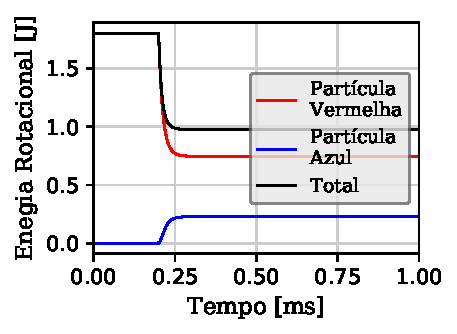
\includegraphics[scale=1]{images/colliding_spheres/dissipative_rotation/rotationalEnergy_small_total_alternative.pdf}
			\caption{}
			\label{subfig:colliding_spheres:dissipative_rotation:rotational_energy}
		\end{subfigure}
		\begin{subfigure}[t]{\smallresultsfigwidth}
			\centering
			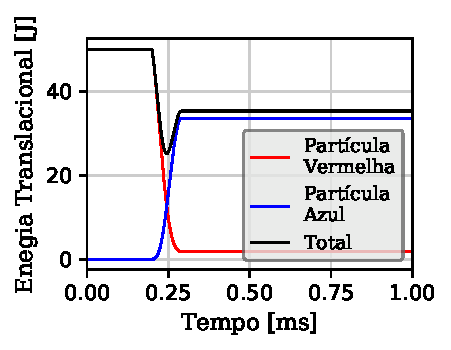
\includegraphics[scale=1]{images/colliding_spheres/dissipative_rotation/translationalEnergy_small_total.pdf}
			\caption{}
			\label{subfig:colliding_spheres:dissipative_rotation:translational_energy}
		\end{subfigure}
		\begin{subfigure}[t]{\smallresultsfigwidth}
			\centering
			\includegraphics[scale=1]{images/colliding_spheres/dissipative_rotation/kineticEnergy_small_total.pdf}
			\caption{}
			\label{subfig:colliding_spheres:dissipative_rotation:kinetic_energy}
		\end{subfigure}
		\begin{subfigure}[t]{\smallresultsfigwidth}
			\centering
			\includegraphics[scale=1]{images/colliding_spheres/dissipative_rotation/coefficient_of_restitution_small.pdf}
			\caption{}
			\label{subfig:colliding_spheres:dissipative_rotation:coefficient_of_restitution}
		\end{subfigure}
	}
	\label{fig:colliding_spheres:dissipative_rotation:energy_and_coefficient_of_restitution_results}
	\sourceMe
\end{figure}

\section{Queda com Arrasto}

Como afirmado na \cref{sec:objectives_and_contributions}, um dos objetivos deste trabalho é possibilitar o uso de interações de naturezas distintas e o acoplamento entre a dinâmica de partículas e a mecânica de fluidos. Assim, esta seção é dedicada a demonstrar a capacidade do simulador de lidar com esse tipo de problema.

Considera-se uma partícula esférica \(\particle\) de raio \(\radius\) e massa \(\mass\) liberada, em repouso, na posição \(\position = \explicitVector{0}{\positiony}{0}\). A partícula sofre a ação da gravidade \(\gravity = \explicitVector{0}{-\gravityScalar}{0}\) com \(\gravityScalar>0\). A esfera é envolvida por ar atmosférico, e, por isso, sofre a ação da força de arrasto durante a sua queda. Essa configuração é representada pela \cref{fig:falling_with_drag}.

\begin{figure}[h]
	\caption{O problema da queda com arrasto.}
	\centering
		\alert{Colocar imagem representando o problema da queda com arrasto}
		% \includegraphics[width=0.65\textwidth]{images/drug_production.png}
	\label{fig:falling_with_drag}
	\source{\alert{Citar fonte}}
\end{figure}

Segundo \citeonline[p. 392]{bib:fox}, a força de arrasto \(\dragForce\) que a partícula sofre é dada por
\begin{equation*}
	\dragForce = \dragCoefficient\ \frac{1}{2}\density\ \projectedArea\ \norm{\velocity} \velocity,
\end{equation*}
em que \(\dragCoefficient\) é o coeficiente de arrasto do par partícula-fluido, \(\density\) é a densidade do ar e \(\projectedArea\) é a área projetada da partícula no plano normal ao seu movimento. Para a esfera, a área projetada é dada por \(\projectedArea = \pi\radius^2\).

O coeficiente de arrasto não é constante, mas varia em função do número de Reynolds \(\reynolds\) definido, para partículas esféricas, como
\begin{equation*}
	\reynolds = \dfrac{\relative{\velocityScalar}\cdot \diameter}{\kinematicViscosity},
\end{equation*}
sendo \(\relative{\velocityScalar}\) a norma da velocidade relativa entre a partícula e o fluido, \(\diameter\), o diâmetro da partícula, e \(\kinematicViscosity\), a viscosidade cinemática do ar. Para o problema em questão, supõe-se que o ar está em repouso, do que segue que a velocidade relativa é idêntica à velocidade \(\velocityScalar\) da partícula.

Apesar dessa dependência, o coeficiente de arrasto apresenta pouca variação para números de Reynolds entre \SI{1000}{} e \SI{300000}{} se se considerarem partículas esféricas lisas \cite[p. 397]{bib:fox}. Para uma esfera de \SI{2}{\centi\meter} de raio, e considerando o ar com viscosidade cinemática de \(\kinematicViscosity = 1,5\cdot 10^{-5}\si[per-mode=symbol]{\square\meter\per\second}\), esses limites correspondem às velocidades de \(\velocityScalar=\SI[per-mode=symbol]{0,375}{\meter\per\second}\) e \(\velocityScalar = \SI[per-mode=symbol]{112,5}{\meter\per\second}\). Por simplicidade, considera-se, aqui, que o coeficiente de arrasto é constante mesmo para velocidades inferiores a \SI[per-mode=symbol]{0,375}{\meter\per\second}. Essa aproximação é razoável tendo em vista que, para o valor da gravidade de \SI[per-mode=symbol]{9,81}{\meter\per\square\second}, a partícula leva aproximadamente \SI{76}{\milli\second} para atingir essa velocidade mínima, sendo que o resto do movimento ocorre dentro da faixa de \(\dragCoefficient\) constante.

Com isso, e a partir dos resultados expostos em \citeonline[p. 397]{bib:fox}, foi fixado o valor \(\dragCoefficient = 0,5\).

A velocidade terminal \(\terminalVelocityScalar\) da partícula é aquela para a qual não ocorre mais a aceleração da partícula. Nessa situação, a força de arrasto se iguala, em módulo, à força peso:
\begin{equation} \label{eq:terminal_velocity}
	\mass\ \gravityScalar = \dragCoefficient\ \frac{1}{2}\density\ \projectedArea\ \terminalVelocityScalar^2 \iff \terminalVelocityScalar = \sqrt{\dfrac{2\ \mass\ \gravityScalar}{\dragCoefficient\ \density\ \projectedArea}},
\end{equation}
e assim se obtém a expressão analítica para a velocidade terminal.

A fim de se simular esse problema, foram considerados os parâmetros expostos na \cref{tab:falling_with_drag:parameters}. 

\begin{table}[h]
\centering
\caption{Parâmetros para o problema da queda com arrasto.}
\label{tab:falling_with_drag:parameters}
\begin{parametersdesc}
	\item{Gravidade}{\gravityScalar = 9,81}{\si[per-mode=symbol]{\metre\per\square\second}}
	\arrayrulecolor[gray]{0.8}\hline
	\item{Massa da partícula}{\mass = 256}{\si\gram}
	\item{Raio da partícula}{\radius = 2}{\si\centi\metre}
	\item{Altura inicial da partícula}{\initial{\positiony} = 3}{\si{\kilo\metre}}
	\item{Velocidade inicial da partícula}{\explicitVector{\initial{\velocityx}}{\initial{\velocityy}}{\initial{\velocityz}} = \explicitVector{0}{0}{0}}{\si[per-mode=symbol]{\metre\per\second}}
	\item{Aceleração inicial da partícula}{\explicitVector{\initial{\accelerationx}}{\initial{\accelerationy}}{\initial{\accelerationz}} = \explicitVector{0}{0}{0}}{\si[per-mode=symbol]{\metre\per\square\second}}
	\arrayrulecolor[gray]{0.8}\hline
	\item{Densidade do ar}{\density = 1}{\si[per-mode=symbol]{\kilogram\per\cubic\meter}}
	\item{Coeficiente de arrasto}{\dragCoefficient = 0,5}{\emptyUnit}
	\arrayrulecolor[gray]{0.8}\hline
	\item{Instante final}{\finalInstant = 40}{\si\second} 
	\item{Passo de tempo}{\Dt = 0,1}{\si\second}
	\item{Ordem de extrapolação}{\taylorOrder = 7}{\emptyUnit}
	\arrayrulecolor{black}
\end{parametersdesc}
\sourceMe 
\end{table}

Com esses valores, foi executada uma simulação, e a altura da partícula em função do tempo foi obtida tal como na \cref{fig:falling_with_drag:height}. A velocidade vertical, por sua vez, está ilustrada na \cref{fig:falling_with_drag:speed}, sendo que a velocidade terminal é calculada analiticamente pela \cref{eq:terminal_velocity}. A energia cinética e a energia mecânica, calculadas de acordo com as \cref{eq:kineticEnergy,eq:mechanicalEnergy}, estão expostas na \cref{fig:falling_with_drag:energy}.

\begin{figure}[h]
	\caption{Solução para a altura da partícula no problema de queda com arrasto.}
	\centering
	\includegraphics[scale=1]{images/falling_with_drag/y_position_small.pdf}
	\label{fig:falling_with_drag:height}
	\sourceMe
\end{figure}

\begin{figure}[htb!]
	\caption{Resultado numérico da velocidade vertical da partícula no problema de queda livre com arrasto, e solução analítica para a velocidade terminal.}
	\centering
	\includegraphics[scale=1]{images/falling_with_drag/y_velocity_normal.pdf}
	\label{fig:falling_with_drag:speed}
	\sourceMe
\end{figure}

\begin{figure}[htb!]
	\caption[Energia cinética e energia mecânica da partícula no problema de queda com arrasto.]{Energia cinética (\subref{subfig:falling_with_drag:kinetic_energy}) e energia mecânica (\subref{subfig:falling_with_drag:mechanical_energy}) da partícula no problema de queda com arrasto.}
	\centering
	\captionsetup[subfloat]{labelfont=bf}
	\subfloat{
		\centering
		\begin{subfigure}[t]{\smallresultsfigwidth}
			\centering
			\includegraphics[scale=1]{images/falling_with_drag/kinetic_energy_small.pdf}
			\caption{}
			\label{subfig:falling_with_drag:kinetic_energy}
		\end{subfigure}
		\begin{subfigure}[t]{\smallresultsfigwidth}
			\centering
			\includegraphics[scale=1]{images/falling_with_drag/mechanical_energy_small.pdf}
			\caption{}
			\label{subfig:falling_with_drag:mechanical_energy}
		\end{subfigure}
	}
	\label{fig:falling_with_drag:energy}
	\sourceMe
\end{figure}

Observa-se que a velocidade da partícula converge para a velocidade terminal prevista analiticamente, evidenciando o correto comportamento do programa mesmo em um problema envolvendo a interação entre fluido e partícula. A energia cinética cresce em função da transformação da energia potencial em movimento. Entretanto esse crescimento é retardado até cessar aproximadamente em \SI{30}{\second} de simulação. A queda na energia mecânica da partícula, por sua vez, pode ser explicada pela dissipação provocada pelo arrasto. Como se observa, a força de arrasto é responsável por dissipar mais de \SI{6}{\kilo\joule} em \SI{40}{\second} de queda.

A importância dessa simulação reside no fato de que, embora o problema considerado seja simples e de fácil solução analítica, ele representa o transporte de informação do fluido para o elemento discreto, como indicado na \cref{sec:discrete_element_method:coupling_with_other_methods}.